\documentclass[twoside]{book}

% Packages required by doxygen
\usepackage{fixltx2e}
\usepackage{calc}
\usepackage{doxygen}
\usepackage[export]{adjustbox} % also loads graphicx
\usepackage{graphicx}
\usepackage[utf8]{inputenc}
\usepackage{makeidx}
\usepackage{multicol}
\usepackage{multirow}
\PassOptionsToPackage{warn}{textcomp}
\usepackage{textcomp}
\usepackage[nointegrals]{wasysym}
\usepackage[table]{xcolor}

% Font selection
\usepackage[T1]{fontenc}
\usepackage[scaled=.90]{helvet}
\usepackage{courier}
\usepackage{amssymb}
\usepackage{sectsty}
\renewcommand{\familydefault}{\sfdefault}
\allsectionsfont{%
  \fontseries{bc}\selectfont%
  \color{darkgray}%
}
\renewcommand{\DoxyLabelFont}{%
  \fontseries{bc}\selectfont%
  \color{darkgray}%
}
\newcommand{\+}{\discretionary{\mbox{\scriptsize$\hookleftarrow$}}{}{}}

% Page & text layout
\usepackage{geometry}
\geometry{%
  a4paper,%
  top=2.5cm,%
  bottom=2.5cm,%
  left=2.5cm,%
  right=2.5cm%
}
\tolerance=750
\hfuzz=15pt
\hbadness=750
\setlength{\emergencystretch}{15pt}
\setlength{\parindent}{0cm}
\setlength{\parskip}{3ex plus 2ex minus 2ex}
\makeatletter
\renewcommand{\paragraph}{%
  \@startsection{paragraph}{4}{0ex}{-1.0ex}{1.0ex}{%
    \normalfont\normalsize\bfseries\SS@parafont%
  }%
}
\renewcommand{\subparagraph}{%
  \@startsection{subparagraph}{5}{0ex}{-1.0ex}{1.0ex}{%
    \normalfont\normalsize\bfseries\SS@subparafont%
  }%
}
\makeatother

% Headers & footers
\usepackage{fancyhdr}
\pagestyle{fancyplain}
\fancyhead[LE]{\fancyplain{}{\bfseries\thepage}}
\fancyhead[CE]{\fancyplain{}{}}
\fancyhead[RE]{\fancyplain{}{\bfseries\leftmark}}
\fancyhead[LO]{\fancyplain{}{\bfseries\rightmark}}
\fancyhead[CO]{\fancyplain{}{}}
\fancyhead[RO]{\fancyplain{}{\bfseries\thepage}}
\fancyfoot[LE]{\fancyplain{}{}}
\fancyfoot[CE]{\fancyplain{}{}}
\fancyfoot[RE]{\fancyplain{}{\bfseries\scriptsize Generated by Doxygen }}
\fancyfoot[LO]{\fancyplain{}{\bfseries\scriptsize Generated by Doxygen }}
\fancyfoot[CO]{\fancyplain{}{}}
\fancyfoot[RO]{\fancyplain{}{}}
\renewcommand{\footrulewidth}{0.4pt}
\renewcommand{\chaptermark}[1]{%
  \markboth{#1}{}%
}
\renewcommand{\sectionmark}[1]{%
  \markright{\thesection\ #1}%
}

% Indices & bibliography
\usepackage{natbib}
\usepackage[titles]{tocloft}
\setcounter{tocdepth}{3}
\setcounter{secnumdepth}{5}
\makeindex

% Hyperlinks (required, but should be loaded last)
\usepackage{ifpdf}
\ifpdf
  \usepackage[pdftex,pagebackref=true]{hyperref}
\else
  \usepackage[ps2pdf,pagebackref=true]{hyperref}
\fi
\hypersetup{%
  colorlinks=true,%
  linkcolor=blue,%
  citecolor=blue,%
  unicode%
}

% Custom commands
\newcommand{\clearemptydoublepage}{%
  \newpage{\pagestyle{empty}\cleardoublepage}%
}

\usepackage{caption}
\captionsetup{labelsep=space,justification=centering,font={bf},singlelinecheck=off,skip=4pt,position=top}

%===== C O N T E N T S =====

\begin{document}

% Titlepage & ToC
\hypersetup{pageanchor=false,
             bookmarksnumbered=true,
             pdfencoding=unicode
            }
\pagenumbering{alph}
\begin{titlepage}
\vspace*{7cm}
\begin{center}%
{\Large Hiss\+Tools F\+FT \\[1ex]\large 1.\+0 }\\
\vspace*{1cm}
{\large Generated by Doxygen 1.8.13}\\
\end{center}
\end{titlepage}
\clearemptydoublepage
\pagenumbering{roman}
\tableofcontents
\clearemptydoublepage
\pagenumbering{arabic}
\hypersetup{pageanchor=true}

%--- Begin generated contents ---
\chapter{Hierarchical Index}
\section{Class Hierarchy}
This inheritance list is sorted roughly, but not completely, alphabetically\+:\begin{DoxyCompactList}
\item \contentsline{section}{Split$<$ T $>$}{\pageref{_h_i_s_s_tools___f_f_t_8h}}{}
\item \contentsline{section}{Split$<$ double $>$}{\pageref{_h_i_s_s_tools___f_f_t_8h}}{}
\begin{DoxyCompactList}
\item \contentsline{section}{F\+F\+T\+\_\+\+S\+P\+L\+I\+T\+\_\+\+C\+O\+M\+P\+L\+E\+X\+\_\+D}{\pageref{struct_double_split}}{}
\end{DoxyCompactList}
\item \contentsline{section}{Split$<$ float $>$}{\pageref{_h_i_s_s_tools___f_f_t_8h}}{}
\begin{DoxyCompactList}
\item \contentsline{section}{F\+F\+T\+\_\+\+S\+P\+L\+I\+T\+\_\+\+C\+O\+M\+P\+L\+E\+X\+\_\+F}{\pageref{struct_float_split}}{}
\end{DoxyCompactList}
\end{DoxyCompactList}

\chapter{Class Index}
\section{Class List}
Here are the classes, structs, unions and interfaces with brief descriptions\+:\begin{DoxyCompactList}
\item\contentsline{section}{\hyperlink{struct_double_setup}{F\+F\+T\+\_\+\+S\+E\+T\+U\+P\+\_\+D} }{\pageref{struct_double_setup}}{}
\item\contentsline{section}{\hyperlink{struct_float_setup}{F\+F\+T\+\_\+\+S\+E\+T\+U\+P\+\_\+F} }{\pageref{struct_float_setup}}{}
\item\contentsline{section}{\hyperlink{struct_double_split}{F\+F\+T\+\_\+\+S\+P\+L\+I\+T\+\_\+\+C\+O\+M\+P\+L\+E\+X\+\_\+D} }{\pageref{struct_double_split}}{}
\item\contentsline{section}{\hyperlink{struct_float_split}{F\+F\+T\+\_\+\+S\+P\+L\+I\+T\+\_\+\+C\+O\+M\+P\+L\+E\+X\+\_\+F} }{\pageref{struct_float_split}}{}
\item\contentsline{section}{\hyperlink{struct_split}{Split$<$ T $>$} }{\pageref{struct_split}}{}
\end{DoxyCompactList}

\chapter{File Index}
\section{File List}
Here is a list of all documented files with brief descriptions\+:\begin{DoxyCompactList}
\item\contentsline{section}{\hyperlink{_h_i_s_s_tools___f_f_t_8h}{H\+I\+S\+S\+Tools\+\_\+\+F\+F\+T.\+h} \\*The main interface for the H\+I\+S\+S\+Tools F\+FT }{\pageref{_h_i_s_s_tools___f_f_t_8h}}{}
\item\contentsline{section}{{\bfseries H\+I\+S\+S\+Tools\+\_\+\+F\+F\+T\+\_\+\+Core.\+h} }{\pageref{_h_i_s_s_tools___f_f_t___core_8h}}{}
\end{DoxyCompactList}

\chapter{Class Documentation}
\hypertarget{struct_double_setup}{}\section{F\+F\+T\+\_\+\+S\+E\+T\+U\+P\+\_\+D Struct Reference}
\label{struct_double_setup}\index{F\+F\+T\+\_\+\+S\+E\+T\+U\+P\+\_\+D@{F\+F\+T\+\_\+\+S\+E\+T\+U\+P\+\_\+D}}


Inherits Setup$<$ T $>$.



\subsection{Detailed Description}
F\+F\+T\+\_\+\+S\+E\+T\+U\+P\+\_\+D is an opaque setup structure for a double-\/precision F\+FT. 

The documentation for this struct was generated from the following file\+:\begin{DoxyCompactItemize}
\item 
F\+F\+T\+\_\+\+Core.\+h\end{DoxyCompactItemize}

\hypertarget{struct_float_setup}{}\section{F\+F\+T\+\_\+\+S\+E\+T\+U\+P\+\_\+F Struct Reference}
\label{struct_float_setup}\index{F\+F\+T\+\_\+\+S\+E\+T\+U\+P\+\_\+F@{F\+F\+T\+\_\+\+S\+E\+T\+U\+P\+\_\+F}}


Inherits Setup$<$ T $>$.



\subsection{Detailed Description}
F\+F\+T\+\_\+\+S\+E\+T\+U\+P\+\_\+F is an opaque setup structure for a single-\/precision F\+FT. 

The documentation for this struct was generated from the following file\+:\begin{DoxyCompactItemize}
\item 
F\+F\+T\+\_\+\+Core.\+h\end{DoxyCompactItemize}

\hypertarget{struct_double_split}{}\section{F\+F\+T\+\_\+\+S\+P\+L\+I\+T\+\_\+\+C\+O\+M\+P\+L\+E\+X\+\_\+D Struct Reference}
\label{struct_double_split}\index{F\+F\+T\+\_\+\+S\+P\+L\+I\+T\+\_\+\+C\+O\+M\+P\+L\+E\+X\+\_\+D@{F\+F\+T\+\_\+\+S\+P\+L\+I\+T\+\_\+\+C\+O\+M\+P\+L\+E\+X\+\_\+D}}
Inheritance diagram for F\+F\+T\+\_\+\+S\+P\+L\+I\+T\+\_\+\+C\+O\+M\+P\+L\+E\+X\+\_\+D\+:\begin{figure}[H]
\begin{center}
\leavevmode
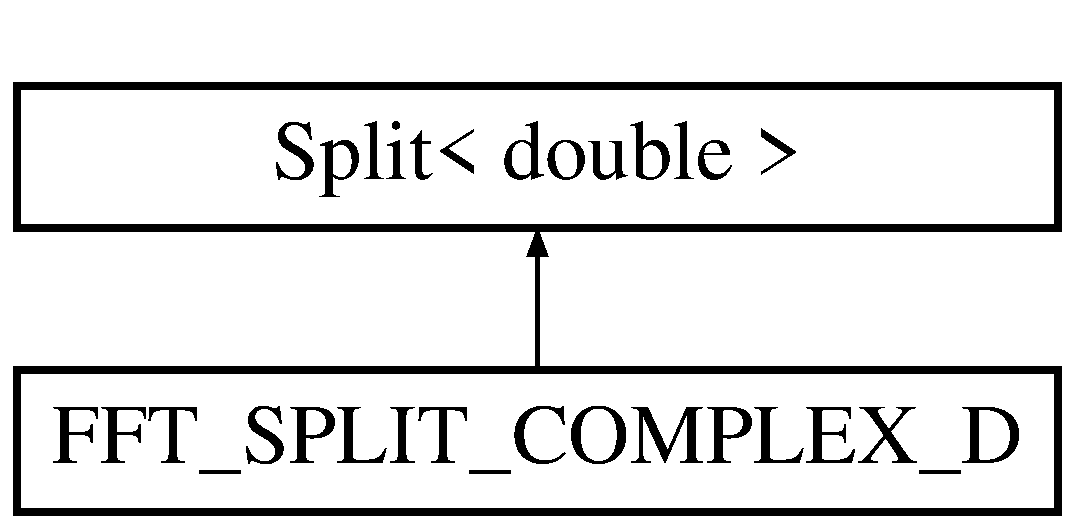
\includegraphics[height=2.000000cm]{struct_double_split}
\end{center}
\end{figure}
\subsection*{Public Attributes}
\begin{DoxyCompactItemize}
\item 
double $\ast$ \hyperlink{_h_i_s_s_tools___f_f_t_8h_aaadcedfa082d6f07b33cd89ea4f19814}{realp}
\item 
double $\ast$ \hyperlink{_h_i_s_s_tools___f_f_t_8h_a21ff23a96abee0c0ed6a2433798c4eac}{imagp}
\end{DoxyCompactItemize}


\subsection{Detailed Description}
F\+F\+T\+\_\+\+S\+P\+L\+I\+T\+\_\+\+C\+O\+M\+P\+L\+E\+X\+\_\+D is a Structure for storing a double-\/precision complex array in split form. 

\subsection{Member Data Documentation}
\mbox{\Hypertarget{_h_i_s_s_tools___f_f_t_8h_aaadcedfa082d6f07b33cd89ea4f19814}\label{_h_i_s_s_tools___f_f_t_8h_aaadcedfa082d6f07b33cd89ea4f19814}} 
\index{Double\+Split@{Double\+Split}!realp@{realp}}
\index{realp@{realp}!Double\+Split@{Double\+Split}}
\subsubsection{\texorpdfstring{realp}{realp}}
{\footnotesize\ttfamily double $\ast$ \hyperlink{_h_i_s_s_tools___f_f_t_8h_struct_split}{Split}$<$ double  $>$\+::realp\hspace{0.3cm}{\ttfamily [inherited]}}

A pointer to the real portion of the data \mbox{\Hypertarget{_h_i_s_s_tools___f_f_t_8h_a21ff23a96abee0c0ed6a2433798c4eac}\label{_h_i_s_s_tools___f_f_t_8h_a21ff23a96abee0c0ed6a2433798c4eac}} 
\index{Double\+Split@{Double\+Split}!imagp@{imagp}}
\index{imagp@{imagp}!Double\+Split@{Double\+Split}}
\subsubsection{\texorpdfstring{imagp}{imagp}}
{\footnotesize\ttfamily double $\ast$ \hyperlink{_h_i_s_s_tools___f_f_t_8h_struct_split}{Split}$<$ double  $>$\+::imagp\hspace{0.3cm}{\ttfamily [inherited]}}

A pointer to the imaginary portion of the data 

The documentation for this struct was generated from the following file\+:\begin{DoxyCompactItemize}
\item 
\hyperlink{_h_i_s_s_tools___f_f_t_8h}{H\+I\+S\+S\+Tools\+\_\+\+F\+F\+T.\+h}\end{DoxyCompactItemize}

\hypertarget{struct_float_split}{}\section{F\+F\+T\+\_\+\+S\+P\+L\+I\+T\+\_\+\+C\+O\+M\+P\+L\+E\+X\+\_\+F Struct Reference}
\label{struct_float_split}\index{F\+F\+T\+\_\+\+S\+P\+L\+I\+T\+\_\+\+C\+O\+M\+P\+L\+E\+X\+\_\+F@{F\+F\+T\+\_\+\+S\+P\+L\+I\+T\+\_\+\+C\+O\+M\+P\+L\+E\+X\+\_\+F}}
Inheritance diagram for F\+F\+T\+\_\+\+S\+P\+L\+I\+T\+\_\+\+C\+O\+M\+P\+L\+E\+X\+\_\+F\+:\begin{figure}[H]
\begin{center}
\leavevmode
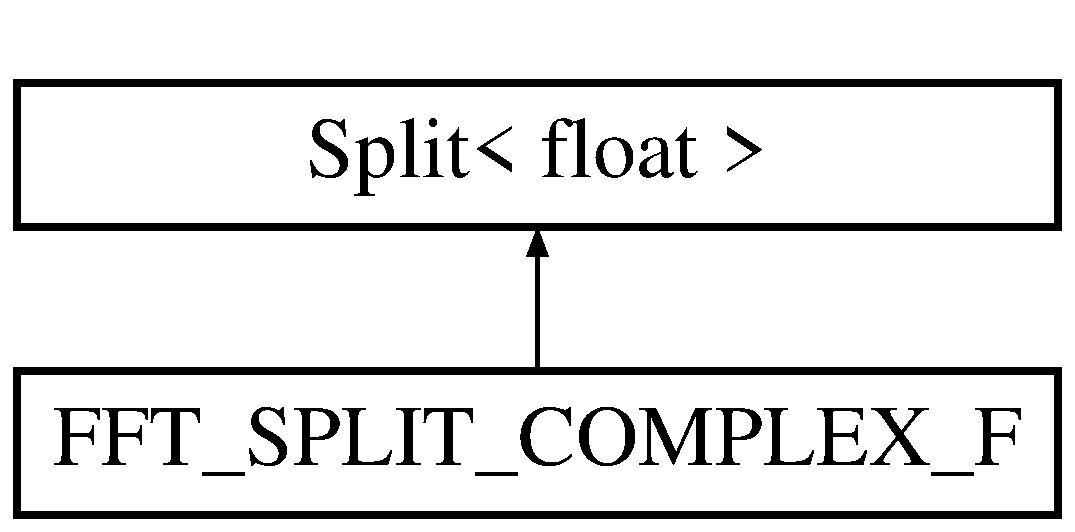
\includegraphics[height=2.000000cm]{struct_float_split}
\end{center}
\end{figure}
\subsection*{Public Attributes}
\begin{DoxyCompactItemize}
\item 
float $\ast$ \hyperlink{_h_i_s_s_tools___f_f_t_8h_aaadcedfa082d6f07b33cd89ea4f19814}{realp}
\item 
float $\ast$ \hyperlink{_h_i_s_s_tools___f_f_t_8h_a21ff23a96abee0c0ed6a2433798c4eac}{imagp}
\end{DoxyCompactItemize}


\subsection{Detailed Description}
F\+F\+T\+\_\+\+S\+P\+L\+I\+T\+\_\+\+C\+O\+M\+P\+L\+E\+X\+\_\+F is a Structure for storing a single-\/precision complex array in split form. 

\subsection{Member Data Documentation}
\mbox{\Hypertarget{_h_i_s_s_tools___f_f_t_8h_aaadcedfa082d6f07b33cd89ea4f19814}\label{_h_i_s_s_tools___f_f_t_8h_aaadcedfa082d6f07b33cd89ea4f19814}} 
\index{Float\+Split@{Float\+Split}!realp@{realp}}
\index{realp@{realp}!Float\+Split@{Float\+Split}}
\subsubsection{\texorpdfstring{realp}{realp}}
{\footnotesize\ttfamily float $\ast$ \hyperlink{_h_i_s_s_tools___f_f_t_8h_struct_split}{Split}$<$ float  $>$\+::realp\hspace{0.3cm}{\ttfamily [inherited]}}

A pointer to the real portion of the data \mbox{\Hypertarget{_h_i_s_s_tools___f_f_t_8h_a21ff23a96abee0c0ed6a2433798c4eac}\label{_h_i_s_s_tools___f_f_t_8h_a21ff23a96abee0c0ed6a2433798c4eac}} 
\index{Float\+Split@{Float\+Split}!imagp@{imagp}}
\index{imagp@{imagp}!Float\+Split@{Float\+Split}}
\subsubsection{\texorpdfstring{imagp}{imagp}}
{\footnotesize\ttfamily float $\ast$ \hyperlink{_h_i_s_s_tools___f_f_t_8h_struct_split}{Split}$<$ float  $>$\+::imagp\hspace{0.3cm}{\ttfamily [inherited]}}

A pointer to the imaginary portion of the data 

The documentation for this struct was generated from the following file\+:\begin{DoxyCompactItemize}
\item 
\hyperlink{_h_i_s_s_tools___f_f_t_8h}{H\+I\+S\+S\+Tools\+\_\+\+F\+F\+T.\+h}\end{DoxyCompactItemize}

\hypertarget{struct_split}{}\section{Split$<$ T $>$ Struct Template Reference}
\label{struct_split}\index{Split$<$ T $>$@{Split$<$ T $>$}}


{\ttfamily \#include $<$H\+I\+S\+S\+Tools\+\_\+\+F\+F\+T.\+h$>$}

\subsection*{Public Attributes}
\begin{DoxyCompactItemize}
\item 
T $\ast$ \hyperlink{struct_split_aaadcedfa082d6f07b33cd89ea4f19814}{realp}
\item 
T $\ast$ \hyperlink{struct_split_a21ff23a96abee0c0ed6a2433798c4eac}{imagp}
\end{DoxyCompactItemize}


\subsection{Detailed Description}
\subsubsection*{template$<$class T$>$\newline
struct Split$<$ T $>$}

\hyperlink{struct_split}{Split} is a \hyperlink{struct_split}{Split} for a double-\/precision F\+FT. 

\subsection{Member Data Documentation}
\mbox{\Hypertarget{struct_split_aaadcedfa082d6f07b33cd89ea4f19814}\label{struct_split_aaadcedfa082d6f07b33cd89ea4f19814}} 
\index{Split@{Split}!realp@{realp}}
\index{realp@{realp}!Split@{Split}}
\subsubsection{\texorpdfstring{realp}{realp}}
{\footnotesize\ttfamily template$<$class T$>$ \\
T$\ast$ \hyperlink{struct_split}{Split}$<$ T $>$\+::realp}

A pointer to the real portion of the data \mbox{\Hypertarget{struct_split_a21ff23a96abee0c0ed6a2433798c4eac}\label{struct_split_a21ff23a96abee0c0ed6a2433798c4eac}} 
\index{Split@{Split}!imagp@{imagp}}
\index{imagp@{imagp}!Split@{Split}}
\subsubsection{\texorpdfstring{imagp}{imagp}}
{\footnotesize\ttfamily template$<$class T$>$ \\
T$\ast$ \hyperlink{struct_split}{Split}$<$ T $>$\+::imagp}

A pointer to the imaginary portion of the data 

The documentation for this struct was generated from the following file\+:\begin{DoxyCompactItemize}
\item 
H\+I\+S\+S\+Tools\+\_\+\+F\+F\+T.\+h\end{DoxyCompactItemize}

\chapter{File Documentation}
\hypertarget{_h_i_s_s_tools___f_f_t_8h}{}\section{H\+I\+S\+S\+Tools\+\_\+\+F\+F\+T.\+h File Reference}
\label{_h_i_s_s_tools___f_f_t_8h}\index{H\+I\+S\+S\+Tools\+\_\+\+F\+F\+T.\+h@{H\+I\+S\+S\+Tools\+\_\+\+F\+F\+T.\+h}}


The main interface for the H\+I\+S\+S\+Tools F\+FT.  


{\ttfamily \#include $<$stdint.\+h$>$}\newline
\subsection*{Classes}
\begin{DoxyCompactItemize}
\item 
struct \hyperlink{_h_i_s_s_tools___f_f_t_8h_struct_split}{Split$<$ T $>$}
\item 
struct \hyperlink{struct_double_split}{F\+F\+T\+\_\+\+S\+P\+L\+I\+T\+\_\+\+C\+O\+M\+P\+L\+E\+X\+\_\+D}
\item 
struct \hyperlink{struct_float_split}{F\+F\+T\+\_\+\+S\+P\+L\+I\+T\+\_\+\+C\+O\+M\+P\+L\+E\+X\+\_\+F}
\end{DoxyCompactItemize}
\subsection*{Macros}
\begin{DoxyCompactItemize}
\item 
\#define \hyperlink{_h_i_s_s_tools___f_f_t_8h_af31c4593411a6c4640544aa7fb57cc6a}{U\+S\+E\+\_\+\+A\+P\+P\+L\+E\+\_\+\+F\+F\+T\+\_\+\+I\+F\+\_\+\+A\+V\+A\+I\+L\+A\+B\+LE}
\end{DoxyCompactItemize}
\subsection*{Typedefs}
\begin{DoxyCompactItemize}
\item 
typedef struct Double\+Setup $\ast$ \hyperlink{_h_i_s_s_tools___f_f_t_8h_a1af7604e4f1f4fe8790c19f9ccc47543}{F\+F\+T\+\_\+\+S\+E\+T\+U\+P\+\_\+D}
\item 
typedef struct Float\+Setup $\ast$ \hyperlink{_h_i_s_s_tools___f_f_t_8h_aa0e1a9e21c0cea49957677ed33c04878}{F\+F\+T\+\_\+\+S\+E\+T\+U\+P\+\_\+F}
\end{DoxyCompactItemize}
\subsection*{Functions}
\begin{DoxyCompactItemize}
\item 
void \hyperlink{_h_i_s_s_tools___f_f_t_8h_adea255b965d708b2922af49e1538dff5}{hisstools\+\_\+create\+\_\+setup} (\hyperlink{_h_i_s_s_tools___f_f_t_8h_a1af7604e4f1f4fe8790c19f9ccc47543}{F\+F\+T\+\_\+\+S\+E\+T\+U\+P\+\_\+D} $\ast$setup, uintptr\+\_\+t max\+\_\+fft\+\_\+log\+\_\+2)
\item 
void \hyperlink{_h_i_s_s_tools___f_f_t_8h_ad2608d5611659d5bbd23c276158cc361}{hisstools\+\_\+create\+\_\+setup} (\hyperlink{_h_i_s_s_tools___f_f_t_8h_aa0e1a9e21c0cea49957677ed33c04878}{F\+F\+T\+\_\+\+S\+E\+T\+U\+P\+\_\+F} $\ast$setup, uintptr\+\_\+t max\+\_\+fft\+\_\+log\+\_\+2)
\item 
void \hyperlink{_h_i_s_s_tools___f_f_t_8h_a300557ff52dd6b5799ea812e7210d7e8}{hisstools\+\_\+destroy\+\_\+setup} (\hyperlink{_h_i_s_s_tools___f_f_t_8h_a1af7604e4f1f4fe8790c19f9ccc47543}{F\+F\+T\+\_\+\+S\+E\+T\+U\+P\+\_\+D} setup)
\item 
void \hyperlink{_h_i_s_s_tools___f_f_t_8h_a3c35cb5a257131181f8cb9ce5d6125a8}{hisstools\+\_\+destroy\+\_\+setup} (\hyperlink{_h_i_s_s_tools___f_f_t_8h_aa0e1a9e21c0cea49957677ed33c04878}{F\+F\+T\+\_\+\+S\+E\+T\+U\+P\+\_\+F} setup)
\item 
void \hyperlink{_h_i_s_s_tools___f_f_t_8h_a3546bf7a638de4dee99ae8cc8cf65105}{hisstools\+\_\+fft} (\hyperlink{_h_i_s_s_tools___f_f_t_8h_a1af7604e4f1f4fe8790c19f9ccc47543}{F\+F\+T\+\_\+\+S\+E\+T\+U\+P\+\_\+D} setup, F\+F\+T\+\_\+\+S\+P\+L\+I\+T\+\_\+\+C\+O\+M\+P\+L\+E\+X\+\_\+D $\ast$input, uintptr\+\_\+t log2n)
\item 
void \hyperlink{_h_i_s_s_tools___f_f_t_8h_a30dff54e3a602cee3d79a7c6fad28be5}{hisstools\+\_\+fft} (\hyperlink{_h_i_s_s_tools___f_f_t_8h_aa0e1a9e21c0cea49957677ed33c04878}{F\+F\+T\+\_\+\+S\+E\+T\+U\+P\+\_\+F} setup, F\+F\+T\+\_\+\+S\+P\+L\+I\+T\+\_\+\+C\+O\+M\+P\+L\+E\+X\+\_\+F $\ast$input, uintptr\+\_\+t log2n)
\item 
void \hyperlink{_h_i_s_s_tools___f_f_t_8h_ae13b19579d4d130c04d347b064ada337}{hisstools\+\_\+rfft} (\hyperlink{_h_i_s_s_tools___f_f_t_8h_a1af7604e4f1f4fe8790c19f9ccc47543}{F\+F\+T\+\_\+\+S\+E\+T\+U\+P\+\_\+D} setup, F\+F\+T\+\_\+\+S\+P\+L\+I\+T\+\_\+\+C\+O\+M\+P\+L\+E\+X\+\_\+D $\ast$input, uintptr\+\_\+t log2n)
\item 
void \hyperlink{_h_i_s_s_tools___f_f_t_8h_a197d9510366d4a5302954b892195f912}{hisstools\+\_\+rfft} (\hyperlink{_h_i_s_s_tools___f_f_t_8h_aa0e1a9e21c0cea49957677ed33c04878}{F\+F\+T\+\_\+\+S\+E\+T\+U\+P\+\_\+F} setup, F\+F\+T\+\_\+\+S\+P\+L\+I\+T\+\_\+\+C\+O\+M\+P\+L\+E\+X\+\_\+F $\ast$input, uintptr\+\_\+t log2n)
\item 
void \hyperlink{_h_i_s_s_tools___f_f_t_8h_a702a07760eed77ff68fba99a03759cb5}{hisstools\+\_\+rfft} (\hyperlink{_h_i_s_s_tools___f_f_t_8h_a1af7604e4f1f4fe8790c19f9ccc47543}{F\+F\+T\+\_\+\+S\+E\+T\+U\+P\+\_\+D} setup, double $\ast$input, F\+F\+T\+\_\+\+S\+P\+L\+I\+T\+\_\+\+C\+O\+M\+P\+L\+E\+X\+\_\+D $\ast$output, uintptr\+\_\+t in\+\_\+length, uintptr\+\_\+t log2n)
\item 
void \hyperlink{_h_i_s_s_tools___f_f_t_8h_a3caecc384eb60d64d5118937351be432}{hisstools\+\_\+rfft} (\hyperlink{_h_i_s_s_tools___f_f_t_8h_aa0e1a9e21c0cea49957677ed33c04878}{F\+F\+T\+\_\+\+S\+E\+T\+U\+P\+\_\+F} setup, float $\ast$input, F\+F\+T\+\_\+\+S\+P\+L\+I\+T\+\_\+\+C\+O\+M\+P\+L\+E\+X\+\_\+F $\ast$output, uintptr\+\_\+t in\+\_\+length, uintptr\+\_\+t log2n)
\item 
void \hyperlink{_h_i_s_s_tools___f_f_t_8h_aaa7613065e6365030ce6620a5a87e78d}{hisstools\+\_\+rfft} (\hyperlink{_h_i_s_s_tools___f_f_t_8h_a1af7604e4f1f4fe8790c19f9ccc47543}{F\+F\+T\+\_\+\+S\+E\+T\+U\+P\+\_\+D} setup, float $\ast$input, F\+F\+T\+\_\+\+S\+P\+L\+I\+T\+\_\+\+C\+O\+M\+P\+L\+E\+X\+\_\+D $\ast$output, uintptr\+\_\+t in\+\_\+length, uintptr\+\_\+t log2n)
\item 
void \hyperlink{_h_i_s_s_tools___f_f_t_8h_a20b8b3e4c94354be25c9d347d08e9e0d}{hisstools\+\_\+ifft} (\hyperlink{_h_i_s_s_tools___f_f_t_8h_a1af7604e4f1f4fe8790c19f9ccc47543}{F\+F\+T\+\_\+\+S\+E\+T\+U\+P\+\_\+D} setup, F\+F\+T\+\_\+\+S\+P\+L\+I\+T\+\_\+\+C\+O\+M\+P\+L\+E\+X\+\_\+D $\ast$input, uintptr\+\_\+t log2n)
\item 
void \hyperlink{_h_i_s_s_tools___f_f_t_8h_a42d9f36a6fea81a22341618672e45c8d}{hisstools\+\_\+ifft} (\hyperlink{_h_i_s_s_tools___f_f_t_8h_aa0e1a9e21c0cea49957677ed33c04878}{F\+F\+T\+\_\+\+S\+E\+T\+U\+P\+\_\+F} setup, F\+F\+T\+\_\+\+S\+P\+L\+I\+T\+\_\+\+C\+O\+M\+P\+L\+E\+X\+\_\+F $\ast$input, uintptr\+\_\+t log2n)
\item 
void \hyperlink{_h_i_s_s_tools___f_f_t_8h_af9319d71f9e550fbd0aa006fe4e03d64}{hisstools\+\_\+rifft} (\hyperlink{_h_i_s_s_tools___f_f_t_8h_a1af7604e4f1f4fe8790c19f9ccc47543}{F\+F\+T\+\_\+\+S\+E\+T\+U\+P\+\_\+D} setup, F\+F\+T\+\_\+\+S\+P\+L\+I\+T\+\_\+\+C\+O\+M\+P\+L\+E\+X\+\_\+D $\ast$input, uintptr\+\_\+t log2n)
\item 
void \hyperlink{_h_i_s_s_tools___f_f_t_8h_af3453a0613a7922e293bc3f3794d639a}{hisstools\+\_\+rifft} (\hyperlink{_h_i_s_s_tools___f_f_t_8h_aa0e1a9e21c0cea49957677ed33c04878}{F\+F\+T\+\_\+\+S\+E\+T\+U\+P\+\_\+F} setup, F\+F\+T\+\_\+\+S\+P\+L\+I\+T\+\_\+\+C\+O\+M\+P\+L\+E\+X\+\_\+F $\ast$input, uintptr\+\_\+t log2n)
\item 
void \hyperlink{_h_i_s_s_tools___f_f_t_8h_a17529a75f59312f44eafb03659a9e5ad}{hisstools\+\_\+rifft} (\hyperlink{_h_i_s_s_tools___f_f_t_8h_a1af7604e4f1f4fe8790c19f9ccc47543}{F\+F\+T\+\_\+\+S\+E\+T\+U\+P\+\_\+D} setup, F\+F\+T\+\_\+\+S\+P\+L\+I\+T\+\_\+\+C\+O\+M\+P\+L\+E\+X\+\_\+D $\ast$input, double $\ast$output, uintptr\+\_\+t log2n)
\item 
void \hyperlink{_h_i_s_s_tools___f_f_t_8h_a5ed8702717390b22495b8ba0ad807ca9}{hisstools\+\_\+rifft} (\hyperlink{_h_i_s_s_tools___f_f_t_8h_aa0e1a9e21c0cea49957677ed33c04878}{F\+F\+T\+\_\+\+S\+E\+T\+U\+P\+\_\+F} setup, F\+F\+T\+\_\+\+S\+P\+L\+I\+T\+\_\+\+C\+O\+M\+P\+L\+E\+X\+\_\+F $\ast$input, float $\ast$output, uintptr\+\_\+t log2n)
\item 
void \hyperlink{_h_i_s_s_tools___f_f_t_8h_a8c201825e1c91a26927e88d03bd1076b}{hisstools\+\_\+unzip\+\_\+zero} (double $\ast$input, F\+F\+T\+\_\+\+S\+P\+L\+I\+T\+\_\+\+C\+O\+M\+P\+L\+E\+X\+\_\+D $\ast$output, uintptr\+\_\+t in\+\_\+length, uintptr\+\_\+t log2n)
\item 
void \hyperlink{_h_i_s_s_tools___f_f_t_8h_a0b60a0d00ec8fb365d452d094b66daf4}{hisstools\+\_\+unzip\+\_\+zero} (float $\ast$input, F\+F\+T\+\_\+\+S\+P\+L\+I\+T\+\_\+\+C\+O\+M\+P\+L\+E\+X\+\_\+F $\ast$output, uintptr\+\_\+t in\+\_\+length, uintptr\+\_\+t log2n)
\item 
void \hyperlink{_h_i_s_s_tools___f_f_t_8h_a859b1bec542ed9bef300b0b122c523b1}{hisstools\+\_\+unzip\+\_\+zero} (float $\ast$input, F\+F\+T\+\_\+\+S\+P\+L\+I\+T\+\_\+\+C\+O\+M\+P\+L\+E\+X\+\_\+D $\ast$output, uintptr\+\_\+t in\+\_\+length, uintptr\+\_\+t log2n)
\item 
void \hyperlink{_h_i_s_s_tools___f_f_t_8h_a86bb02a8d1d00a16d42a5bdbbbd23e97}{hisstools\+\_\+unzip} (double $\ast$input, F\+F\+T\+\_\+\+S\+P\+L\+I\+T\+\_\+\+C\+O\+M\+P\+L\+E\+X\+\_\+D $\ast$output, uintptr\+\_\+t log2n)
\item 
void \hyperlink{_h_i_s_s_tools___f_f_t_8h_a1456a40467658dcbf5cbb7d062fa0562}{hisstools\+\_\+unzip} (float $\ast$input, F\+F\+T\+\_\+\+S\+P\+L\+I\+T\+\_\+\+C\+O\+M\+P\+L\+E\+X\+\_\+F $\ast$output, uintptr\+\_\+t log2n)
\item 
void \hyperlink{_h_i_s_s_tools___f_f_t_8h_af8950d25a31ea0a1427da1705d4c91cd}{hisstools\+\_\+zip} (F\+F\+T\+\_\+\+S\+P\+L\+I\+T\+\_\+\+C\+O\+M\+P\+L\+E\+X\+\_\+D $\ast$input, double $\ast$output, uintptr\+\_\+t log2n)
\item 
void \hyperlink{_h_i_s_s_tools___f_f_t_8h_a107e1cea7431f4de930a9ef2c01f7ca9}{hisstools\+\_\+zip} (F\+F\+T\+\_\+\+S\+P\+L\+I\+T\+\_\+\+C\+O\+M\+P\+L\+E\+X\+\_\+F $\ast$input, float $\ast$output, uintptr\+\_\+t log2n)
\end{DoxyCompactItemize}


\subsection{Detailed Description}
The main interface for the H\+I\+S\+S\+Tools F\+FT. 

The F\+FT is compatiable with the F\+FT routines provided by Apple\textquotesingle{}s v\+D\+SP library and can be configured to use this fast F\+FT when available. 

\subsection{Class Documentation}
\index{Split@{Split}}\label{struct_split}
\Hypertarget{_h_i_s_s_tools___f_f_t_8h_struct_split}
\subsubsection{struct Split}
\subsubsection*{template$<$class T$>$\newline
struct Split$<$ T $>$}

\hyperlink{_h_i_s_s_tools___f_f_t_8h_struct_split}{Split} is a \hyperlink{_h_i_s_s_tools___f_f_t_8h_struct_split}{Split} for a double-\/precision F\+FT. \begin{DoxyFields}{Class Members}
\mbox{\Hypertarget{_h_i_s_s_tools___f_f_t_8h_aaadcedfa082d6f07b33cd89ea4f19814}\label{_h_i_s_s_tools___f_f_t_8h_aaadcedfa082d6f07b33cd89ea4f19814}} 
T $\ast$&
realp&
A pointer to the real portion of the data \\
\hline

\mbox{\Hypertarget{_h_i_s_s_tools___f_f_t_8h_a21ff23a96abee0c0ed6a2433798c4eac}\label{_h_i_s_s_tools___f_f_t_8h_a21ff23a96abee0c0ed6a2433798c4eac}} 
T $\ast$&
imagp&
A pointer to the imaginary portion of the data \\
\hline

\end{DoxyFields}


\subsection{Macro Definition Documentation}
\mbox{\Hypertarget{_h_i_s_s_tools___f_f_t_8h_af31c4593411a6c4640544aa7fb57cc6a}\label{_h_i_s_s_tools___f_f_t_8h_af31c4593411a6c4640544aa7fb57cc6a}} 
\index{H\+I\+S\+S\+Tools\+\_\+\+F\+F\+T.\+h@{H\+I\+S\+S\+Tools\+\_\+\+F\+F\+T.\+h}!U\+S\+E\+\_\+\+A\+P\+P\+L\+E\+\_\+\+F\+F\+T\+\_\+\+I\+F\+\_\+\+A\+V\+A\+I\+L\+A\+B\+LE@{U\+S\+E\+\_\+\+A\+P\+P\+L\+E\+\_\+\+F\+F\+T\+\_\+\+I\+F\+\_\+\+A\+V\+A\+I\+L\+A\+B\+LE}}
\index{U\+S\+E\+\_\+\+A\+P\+P\+L\+E\+\_\+\+F\+F\+T\+\_\+\+I\+F\+\_\+\+A\+V\+A\+I\+L\+A\+B\+LE@{U\+S\+E\+\_\+\+A\+P\+P\+L\+E\+\_\+\+F\+F\+T\+\_\+\+I\+F\+\_\+\+A\+V\+A\+I\+L\+A\+B\+LE}!H\+I\+S\+S\+Tools\+\_\+\+F\+F\+T.\+h@{H\+I\+S\+S\+Tools\+\_\+\+F\+F\+T.\+h}}
\subsubsection{\texorpdfstring{U\+S\+E\+\_\+\+A\+P\+P\+L\+E\+\_\+\+F\+F\+T\+\_\+\+I\+F\+\_\+\+A\+V\+A\+I\+L\+A\+B\+LE}{USE\_APPLE\_FFT\_IF\_AVAILABLE}}
{\footnotesize\ttfamily \#define U\+S\+E\+\_\+\+A\+P\+P\+L\+E\+\_\+\+F\+F\+T\+\_\+\+I\+F\+\_\+\+A\+V\+A\+I\+L\+A\+B\+LE}

The U\+S\+E\+\_\+\+A\+P\+P\+L\+E\+\_\+\+F\+F\+T\+\_\+\+I\+F\+\_\+\+A\+V\+A\+I\+L\+A\+B\+LE preprocessor command instructs the H\+I\+S\+S\+Tools F\+FT to use the Apple F\+FT when available. Comment out this definition if you don\textquotesingle{}t wish to use the Apple F\+FT when available. This option is enabled by default. You must link against the Accelerate framework to compile with this functionality under Mac OS. 

\subsection{Typedef Documentation}
\mbox{\Hypertarget{_h_i_s_s_tools___f_f_t_8h_a1af7604e4f1f4fe8790c19f9ccc47543}\label{_h_i_s_s_tools___f_f_t_8h_a1af7604e4f1f4fe8790c19f9ccc47543}} 
\index{H\+I\+S\+S\+Tools\+\_\+\+F\+F\+T.\+h@{H\+I\+S\+S\+Tools\+\_\+\+F\+F\+T.\+h}!F\+F\+T\+\_\+\+S\+E\+T\+U\+P\+\_\+D@{F\+F\+T\+\_\+\+S\+E\+T\+U\+P\+\_\+D}}
\index{F\+F\+T\+\_\+\+S\+E\+T\+U\+P\+\_\+D@{F\+F\+T\+\_\+\+S\+E\+T\+U\+P\+\_\+D}!H\+I\+S\+S\+Tools\+\_\+\+F\+F\+T.\+h@{H\+I\+S\+S\+Tools\+\_\+\+F\+F\+T.\+h}}
\subsubsection{\texorpdfstring{F\+F\+T\+\_\+\+S\+E\+T\+U\+P\+\_\+D}{FFT\_SETUP\_D}}
{\footnotesize\ttfamily typedef struct Double\+Setup$\ast$ \hyperlink{_h_i_s_s_tools___f_f_t_8h_a1af7604e4f1f4fe8790c19f9ccc47543}{F\+F\+T\+\_\+\+S\+E\+T\+U\+P\+\_\+D}}

F\+F\+T\+\_\+\+S\+E\+T\+U\+P\+\_\+D is an opaque setup structure for a double-\/precision F\+FT. \mbox{\Hypertarget{_h_i_s_s_tools___f_f_t_8h_aa0e1a9e21c0cea49957677ed33c04878}\label{_h_i_s_s_tools___f_f_t_8h_aa0e1a9e21c0cea49957677ed33c04878}} 
\index{H\+I\+S\+S\+Tools\+\_\+\+F\+F\+T.\+h@{H\+I\+S\+S\+Tools\+\_\+\+F\+F\+T.\+h}!F\+F\+T\+\_\+\+S\+E\+T\+U\+P\+\_\+F@{F\+F\+T\+\_\+\+S\+E\+T\+U\+P\+\_\+F}}
\index{F\+F\+T\+\_\+\+S\+E\+T\+U\+P\+\_\+F@{F\+F\+T\+\_\+\+S\+E\+T\+U\+P\+\_\+F}!H\+I\+S\+S\+Tools\+\_\+\+F\+F\+T.\+h@{H\+I\+S\+S\+Tools\+\_\+\+F\+F\+T.\+h}}
\subsubsection{\texorpdfstring{F\+F\+T\+\_\+\+S\+E\+T\+U\+P\+\_\+F}{FFT\_SETUP\_F}}
{\footnotesize\ttfamily typedef struct Float\+Setup$\ast$ \hyperlink{_h_i_s_s_tools___f_f_t_8h_aa0e1a9e21c0cea49957677ed33c04878}{F\+F\+T\+\_\+\+S\+E\+T\+U\+P\+\_\+F}}

F\+F\+T\+\_\+\+S\+E\+T\+U\+P\+\_\+F is an opaque setup structure for a single-\/precision F\+FT. 

\subsection{Function Documentation}
\mbox{\Hypertarget{_h_i_s_s_tools___f_f_t_8h_adea255b965d708b2922af49e1538dff5}\label{_h_i_s_s_tools___f_f_t_8h_adea255b965d708b2922af49e1538dff5}} 
\index{H\+I\+S\+S\+Tools\+\_\+\+F\+F\+T.\+h@{H\+I\+S\+S\+Tools\+\_\+\+F\+F\+T.\+h}!hisstools\+\_\+create\+\_\+setup@{hisstools\+\_\+create\+\_\+setup}}
\index{hisstools\+\_\+create\+\_\+setup@{hisstools\+\_\+create\+\_\+setup}!H\+I\+S\+S\+Tools\+\_\+\+F\+F\+T.\+h@{H\+I\+S\+S\+Tools\+\_\+\+F\+F\+T.\+h}}
\subsubsection{\texorpdfstring{hisstools\+\_\+create\+\_\+setup()}{hisstools\_create\_setup()}\hspace{0.1cm}{\footnotesize\ttfamily [1/2]}}
{\footnotesize\ttfamily void hisstools\+\_\+create\+\_\+setup (\begin{DoxyParamCaption}\item[{\hyperlink{_h_i_s_s_tools___f_f_t_8h_a1af7604e4f1f4fe8790c19f9ccc47543}{F\+F\+T\+\_\+\+S\+E\+T\+U\+P\+\_\+D} $\ast$}]{setup,  }\item[{uintptr\+\_\+t}]{max\+\_\+fft\+\_\+log\+\_\+2 }\end{DoxyParamCaption})}

\hyperlink{_h_i_s_s_tools___f_f_t_8h_adea255b965d708b2922af49e1538dff5}{hisstools\+\_\+create\+\_\+setup()} creates an F\+FT setup suitable for double-\/precision F\+F\+Ts and i\+F\+F\+Ts up to a maximum specified size.


\begin{DoxyParams}{Parameters}
{\em setup} & A pointer to an uninitialised F\+F\+T\+\_\+\+S\+E\+T\+U\+P\+\_\+D. \\
\hline
{\em max\+\_\+fft\+\_\+log\+\_\+2} & The log base 2 of the F\+FT size of the maimum F\+FT size you wish to support..\\
\hline
\end{DoxyParams}
\begin{DoxyRemark}{Remarks}
On return the object pointed to by setup will be intialsed, 
\end{DoxyRemark}
\mbox{\Hypertarget{_h_i_s_s_tools___f_f_t_8h_ad2608d5611659d5bbd23c276158cc361}\label{_h_i_s_s_tools___f_f_t_8h_ad2608d5611659d5bbd23c276158cc361}} 
\index{H\+I\+S\+S\+Tools\+\_\+\+F\+F\+T.\+h@{H\+I\+S\+S\+Tools\+\_\+\+F\+F\+T.\+h}!hisstools\+\_\+create\+\_\+setup@{hisstools\+\_\+create\+\_\+setup}}
\index{hisstools\+\_\+create\+\_\+setup@{hisstools\+\_\+create\+\_\+setup}!H\+I\+S\+S\+Tools\+\_\+\+F\+F\+T.\+h@{H\+I\+S\+S\+Tools\+\_\+\+F\+F\+T.\+h}}
\subsubsection{\texorpdfstring{hisstools\+\_\+create\+\_\+setup()}{hisstools\_create\_setup()}\hspace{0.1cm}{\footnotesize\ttfamily [2/2]}}
{\footnotesize\ttfamily void hisstools\+\_\+create\+\_\+setup (\begin{DoxyParamCaption}\item[{\hyperlink{_h_i_s_s_tools___f_f_t_8h_aa0e1a9e21c0cea49957677ed33c04878}{F\+F\+T\+\_\+\+S\+E\+T\+U\+P\+\_\+F} $\ast$}]{setup,  }\item[{uintptr\+\_\+t}]{max\+\_\+fft\+\_\+log\+\_\+2 }\end{DoxyParamCaption})}

\hyperlink{_h_i_s_s_tools___f_f_t_8h_adea255b965d708b2922af49e1538dff5}{hisstools\+\_\+create\+\_\+setup()} creates an F\+FT setup suitable for single-\/precision F\+F\+Ts and i\+F\+F\+Ts up to a maximum specified size.


\begin{DoxyParams}{Parameters}
{\em setup} & A pointer to an uninitialised F\+F\+T\+\_\+\+S\+E\+T\+U\+P\+\_\+F. \\
\hline
{\em max\+\_\+fft\+\_\+log\+\_\+2} & The log base 2 of the F\+FT size of the maimum F\+FT size you wish to support..\\
\hline
\end{DoxyParams}
\begin{DoxyRemark}{Remarks}
On return the object pointed to by setup will be intialsed, 
\end{DoxyRemark}
\mbox{\Hypertarget{_h_i_s_s_tools___f_f_t_8h_a300557ff52dd6b5799ea812e7210d7e8}\label{_h_i_s_s_tools___f_f_t_8h_a300557ff52dd6b5799ea812e7210d7e8}} 
\index{H\+I\+S\+S\+Tools\+\_\+\+F\+F\+T.\+h@{H\+I\+S\+S\+Tools\+\_\+\+F\+F\+T.\+h}!hisstools\+\_\+destroy\+\_\+setup@{hisstools\+\_\+destroy\+\_\+setup}}
\index{hisstools\+\_\+destroy\+\_\+setup@{hisstools\+\_\+destroy\+\_\+setup}!H\+I\+S\+S\+Tools\+\_\+\+F\+F\+T.\+h@{H\+I\+S\+S\+Tools\+\_\+\+F\+F\+T.\+h}}
\subsubsection{\texorpdfstring{hisstools\+\_\+destroy\+\_\+setup()}{hisstools\_destroy\_setup()}\hspace{0.1cm}{\footnotesize\ttfamily [1/2]}}
{\footnotesize\ttfamily void hisstools\+\_\+destroy\+\_\+setup (\begin{DoxyParamCaption}\item[{\hyperlink{_h_i_s_s_tools___f_f_t_8h_a1af7604e4f1f4fe8790c19f9ccc47543}{F\+F\+T\+\_\+\+S\+E\+T\+U\+P\+\_\+D}}]{setup }\end{DoxyParamCaption})}

\hyperlink{_h_i_s_s_tools___f_f_t_8h_a300557ff52dd6b5799ea812e7210d7e8}{hisstools\+\_\+destroy\+\_\+setup()} destroys a double-\/precision F\+FT setup.


\begin{DoxyParams}{Parameters}
{\em setup} & A F\+F\+T\+\_\+\+S\+E\+T\+U\+P\+\_\+D (double-\/precision setup).\\
\hline
\end{DoxyParams}
\begin{DoxyRemark}{Remarks}
After calling this routine the setup is destroyed. 
\end{DoxyRemark}
\mbox{\Hypertarget{_h_i_s_s_tools___f_f_t_8h_a3c35cb5a257131181f8cb9ce5d6125a8}\label{_h_i_s_s_tools___f_f_t_8h_a3c35cb5a257131181f8cb9ce5d6125a8}} 
\index{H\+I\+S\+S\+Tools\+\_\+\+F\+F\+T.\+h@{H\+I\+S\+S\+Tools\+\_\+\+F\+F\+T.\+h}!hisstools\+\_\+destroy\+\_\+setup@{hisstools\+\_\+destroy\+\_\+setup}}
\index{hisstools\+\_\+destroy\+\_\+setup@{hisstools\+\_\+destroy\+\_\+setup}!H\+I\+S\+S\+Tools\+\_\+\+F\+F\+T.\+h@{H\+I\+S\+S\+Tools\+\_\+\+F\+F\+T.\+h}}
\subsubsection{\texorpdfstring{hisstools\+\_\+destroy\+\_\+setup()}{hisstools\_destroy\_setup()}\hspace{0.1cm}{\footnotesize\ttfamily [2/2]}}
{\footnotesize\ttfamily void hisstools\+\_\+destroy\+\_\+setup (\begin{DoxyParamCaption}\item[{\hyperlink{_h_i_s_s_tools___f_f_t_8h_aa0e1a9e21c0cea49957677ed33c04878}{F\+F\+T\+\_\+\+S\+E\+T\+U\+P\+\_\+F}}]{setup }\end{DoxyParamCaption})}

\hyperlink{_h_i_s_s_tools___f_f_t_8h_a300557ff52dd6b5799ea812e7210d7e8}{hisstools\+\_\+destroy\+\_\+setup()} destroys a single-\/precision F\+FT setup.


\begin{DoxyParams}{Parameters}
{\em setup} & A F\+F\+T\+\_\+\+S\+E\+T\+U\+P\+\_\+F (single-\/precision setup).\\
\hline
\end{DoxyParams}
\begin{DoxyRemark}{Remarks}
After calling this routine the setup is destroyed. 
\end{DoxyRemark}
\mbox{\Hypertarget{_h_i_s_s_tools___f_f_t_8h_a3546bf7a638de4dee99ae8cc8cf65105}\label{_h_i_s_s_tools___f_f_t_8h_a3546bf7a638de4dee99ae8cc8cf65105}} 
\index{H\+I\+S\+S\+Tools\+\_\+\+F\+F\+T.\+h@{H\+I\+S\+S\+Tools\+\_\+\+F\+F\+T.\+h}!hisstools\+\_\+fft@{hisstools\+\_\+fft}}
\index{hisstools\+\_\+fft@{hisstools\+\_\+fft}!H\+I\+S\+S\+Tools\+\_\+\+F\+F\+T.\+h@{H\+I\+S\+S\+Tools\+\_\+\+F\+F\+T.\+h}}
\subsubsection{\texorpdfstring{hisstools\+\_\+fft()}{hisstools\_fft()}\hspace{0.1cm}{\footnotesize\ttfamily [1/2]}}
{\footnotesize\ttfamily void hisstools\+\_\+fft (\begin{DoxyParamCaption}\item[{\hyperlink{_h_i_s_s_tools___f_f_t_8h_a1af7604e4f1f4fe8790c19f9ccc47543}{F\+F\+T\+\_\+\+S\+E\+T\+U\+P\+\_\+D}}]{setup,  }\item[{F\+F\+T\+\_\+\+S\+P\+L\+I\+T\+\_\+\+C\+O\+M\+P\+L\+E\+X\+\_\+D $\ast$}]{input,  }\item[{uintptr\+\_\+t}]{log2n }\end{DoxyParamCaption})}

\hyperlink{_h_i_s_s_tools___f_f_t_8h_a3546bf7a638de4dee99ae8cc8cf65105}{hisstools\+\_\+fft()} performs an in-\/place complex Fast Fourier Transform.


\begin{DoxyParams}{Parameters}
{\em setup} & A F\+F\+T\+\_\+\+S\+E\+T\+U\+P\+\_\+D that has been created to deal with an appropriate maximum size of F\+FT. \\
\hline
{\em input} & A pointer to a F\+F\+T\+\_\+\+S\+P\+L\+I\+T\+\_\+\+C\+O\+M\+P\+L\+E\+X\+\_\+D structure containing the complex input. \\
\hline
{\em log2n} & The log base 2 of the F\+FT size.\\
\hline
\end{DoxyParams}
\begin{DoxyRemark}{Remarks}
The F\+FT may be performed with either scalar or S\+I\+MD instructions. S\+I\+MD instuctions will be used when the pointers within the F\+F\+T\+\_\+\+S\+P\+L\+I\+T\+\_\+\+C\+O\+M\+P\+L\+E\+X\+\_\+D are sixteen byte aligned 
\end{DoxyRemark}
\mbox{\Hypertarget{_h_i_s_s_tools___f_f_t_8h_a30dff54e3a602cee3d79a7c6fad28be5}\label{_h_i_s_s_tools___f_f_t_8h_a30dff54e3a602cee3d79a7c6fad28be5}} 
\index{H\+I\+S\+S\+Tools\+\_\+\+F\+F\+T.\+h@{H\+I\+S\+S\+Tools\+\_\+\+F\+F\+T.\+h}!hisstools\+\_\+fft@{hisstools\+\_\+fft}}
\index{hisstools\+\_\+fft@{hisstools\+\_\+fft}!H\+I\+S\+S\+Tools\+\_\+\+F\+F\+T.\+h@{H\+I\+S\+S\+Tools\+\_\+\+F\+F\+T.\+h}}
\subsubsection{\texorpdfstring{hisstools\+\_\+fft()}{hisstools\_fft()}\hspace{0.1cm}{\footnotesize\ttfamily [2/2]}}
{\footnotesize\ttfamily void hisstools\+\_\+fft (\begin{DoxyParamCaption}\item[{\hyperlink{_h_i_s_s_tools___f_f_t_8h_aa0e1a9e21c0cea49957677ed33c04878}{F\+F\+T\+\_\+\+S\+E\+T\+U\+P\+\_\+F}}]{setup,  }\item[{F\+F\+T\+\_\+\+S\+P\+L\+I\+T\+\_\+\+C\+O\+M\+P\+L\+E\+X\+\_\+F $\ast$}]{input,  }\item[{uintptr\+\_\+t}]{log2n }\end{DoxyParamCaption})}

\hyperlink{_h_i_s_s_tools___f_f_t_8h_a3546bf7a638de4dee99ae8cc8cf65105}{hisstools\+\_\+fft()} performs an in-\/place complex Fast Fourier Transform.


\begin{DoxyParams}{Parameters}
{\em setup} & A F\+F\+T\+\_\+\+S\+E\+T\+U\+P\+\_\+F that has been created to deal with an appropriate maximum size of F\+FT. \\
\hline
{\em input} & A pointer to a F\+F\+T\+\_\+\+S\+P\+L\+I\+T\+\_\+\+C\+O\+M\+P\+L\+E\+X\+\_\+F structure containing the complex input. \\
\hline
{\em log2n} & The log base 2 of the F\+FT size.\\
\hline
\end{DoxyParams}
\begin{DoxyRemark}{Remarks}
The F\+FT may be performed with scalar or S\+I\+MD instructions. S\+I\+MD instuctions will be used when the pointers within the F\+F\+T\+\_\+\+S\+P\+L\+I\+T\+\_\+\+C\+O\+M\+P\+L\+E\+X\+\_\+D are sixteen byte aligned. 
\end{DoxyRemark}
\mbox{\Hypertarget{_h_i_s_s_tools___f_f_t_8h_ae13b19579d4d130c04d347b064ada337}\label{_h_i_s_s_tools___f_f_t_8h_ae13b19579d4d130c04d347b064ada337}} 
\index{H\+I\+S\+S\+Tools\+\_\+\+F\+F\+T.\+h@{H\+I\+S\+S\+Tools\+\_\+\+F\+F\+T.\+h}!hisstools\+\_\+rfft@{hisstools\+\_\+rfft}}
\index{hisstools\+\_\+rfft@{hisstools\+\_\+rfft}!H\+I\+S\+S\+Tools\+\_\+\+F\+F\+T.\+h@{H\+I\+S\+S\+Tools\+\_\+\+F\+F\+T.\+h}}
\subsubsection{\texorpdfstring{hisstools\+\_\+rfft()}{hisstools\_rfft()}\hspace{0.1cm}{\footnotesize\ttfamily [1/5]}}
{\footnotesize\ttfamily void hisstools\+\_\+rfft (\begin{DoxyParamCaption}\item[{\hyperlink{_h_i_s_s_tools___f_f_t_8h_a1af7604e4f1f4fe8790c19f9ccc47543}{F\+F\+T\+\_\+\+S\+E\+T\+U\+P\+\_\+D}}]{setup,  }\item[{F\+F\+T\+\_\+\+S\+P\+L\+I\+T\+\_\+\+C\+O\+M\+P\+L\+E\+X\+\_\+D $\ast$}]{input,  }\item[{uintptr\+\_\+t}]{log2n }\end{DoxyParamCaption})}

\hyperlink{_h_i_s_s_tools___f_f_t_8h_ae13b19579d4d130c04d347b064ada337}{hisstools\+\_\+rfft()} performs an in-\/place real Fast Fourier Transform.


\begin{DoxyParams}{Parameters}
{\em setup} & A F\+F\+T\+\_\+\+S\+E\+T\+U\+P\+\_\+D that has been created to deal with an appropriate maximum size of F\+FT. \\
\hline
{\em input} & A pointer to a F\+F\+T\+\_\+\+S\+P\+L\+I\+T\+\_\+\+C\+O\+M\+P\+L\+E\+X\+\_\+D structure containing a complex input. \\
\hline
{\em log2n} & The log base 2 of the F\+FT size.\\
\hline
\end{DoxyParams}
\begin{DoxyRemark}{Remarks}
The F\+FT may be performed with either scalar or S\+I\+MD instructions. S\+I\+MD instuctions will be used when the pointers within the F\+F\+T\+\_\+\+S\+P\+L\+I\+T\+\_\+\+C\+O\+M\+P\+L\+E\+X\+\_\+D are sixteen byte aligned. Note that the input should first be unzipped into the complex input structure using \hyperlink{_h_i_s_s_tools___f_f_t_8h_a86bb02a8d1d00a16d42a5bdbbbd23e97}{hisstools\+\_\+unzip()} or hisstools\+\_\+unzip\+\_\+zero). 
\end{DoxyRemark}
\mbox{\Hypertarget{_h_i_s_s_tools___f_f_t_8h_a197d9510366d4a5302954b892195f912}\label{_h_i_s_s_tools___f_f_t_8h_a197d9510366d4a5302954b892195f912}} 
\index{H\+I\+S\+S\+Tools\+\_\+\+F\+F\+T.\+h@{H\+I\+S\+S\+Tools\+\_\+\+F\+F\+T.\+h}!hisstools\+\_\+rfft@{hisstools\+\_\+rfft}}
\index{hisstools\+\_\+rfft@{hisstools\+\_\+rfft}!H\+I\+S\+S\+Tools\+\_\+\+F\+F\+T.\+h@{H\+I\+S\+S\+Tools\+\_\+\+F\+F\+T.\+h}}
\subsubsection{\texorpdfstring{hisstools\+\_\+rfft()}{hisstools\_rfft()}\hspace{0.1cm}{\footnotesize\ttfamily [2/5]}}
{\footnotesize\ttfamily void hisstools\+\_\+rfft (\begin{DoxyParamCaption}\item[{\hyperlink{_h_i_s_s_tools___f_f_t_8h_aa0e1a9e21c0cea49957677ed33c04878}{F\+F\+T\+\_\+\+S\+E\+T\+U\+P\+\_\+F}}]{setup,  }\item[{F\+F\+T\+\_\+\+S\+P\+L\+I\+T\+\_\+\+C\+O\+M\+P\+L\+E\+X\+\_\+F $\ast$}]{input,  }\item[{uintptr\+\_\+t}]{log2n }\end{DoxyParamCaption})}

\hyperlink{_h_i_s_s_tools___f_f_t_8h_ae13b19579d4d130c04d347b064ada337}{hisstools\+\_\+rfft()} performs an in-\/place real Fast Fourier Transform.


\begin{DoxyParams}{Parameters}
{\em setup} & A F\+F\+T\+\_\+\+S\+E\+T\+U\+P\+\_\+F that has been created to deal with an appropriate maximum size of F\+FT. \\
\hline
{\em input} & A pointer to a F\+F\+T\+\_\+\+S\+P\+L\+I\+T\+\_\+\+C\+O\+M\+P\+L\+E\+X\+\_\+F structure containing a complex input. \\
\hline
{\em log2n} & The log base 2 of the F\+FT size.\\
\hline
\end{DoxyParams}
\begin{DoxyRemark}{Remarks}
The F\+FT may be performed with either scalar or S\+I\+MD instructions. S\+I\+MD instuctions will be used when the pointers within the F\+F\+T\+\_\+\+S\+P\+L\+I\+T\+\_\+\+C\+O\+M\+P\+L\+E\+X\+\_\+D are sixteen byte aligned. Note that the input should first be unzipped into the complex input structure using \hyperlink{_h_i_s_s_tools___f_f_t_8h_a86bb02a8d1d00a16d42a5bdbbbd23e97}{hisstools\+\_\+unzip()} or hisstools\+\_\+unzip\+\_\+zero). 
\end{DoxyRemark}
\mbox{\Hypertarget{_h_i_s_s_tools___f_f_t_8h_a702a07760eed77ff68fba99a03759cb5}\label{_h_i_s_s_tools___f_f_t_8h_a702a07760eed77ff68fba99a03759cb5}} 
\index{H\+I\+S\+S\+Tools\+\_\+\+F\+F\+T.\+h@{H\+I\+S\+S\+Tools\+\_\+\+F\+F\+T.\+h}!hisstools\+\_\+rfft@{hisstools\+\_\+rfft}}
\index{hisstools\+\_\+rfft@{hisstools\+\_\+rfft}!H\+I\+S\+S\+Tools\+\_\+\+F\+F\+T.\+h@{H\+I\+S\+S\+Tools\+\_\+\+F\+F\+T.\+h}}
\subsubsection{\texorpdfstring{hisstools\+\_\+rfft()}{hisstools\_rfft()}\hspace{0.1cm}{\footnotesize\ttfamily [3/5]}}
{\footnotesize\ttfamily void hisstools\+\_\+rfft (\begin{DoxyParamCaption}\item[{\hyperlink{_h_i_s_s_tools___f_f_t_8h_a1af7604e4f1f4fe8790c19f9ccc47543}{F\+F\+T\+\_\+\+S\+E\+T\+U\+P\+\_\+D}}]{setup,  }\item[{double $\ast$}]{input,  }\item[{F\+F\+T\+\_\+\+S\+P\+L\+I\+T\+\_\+\+C\+O\+M\+P\+L\+E\+X\+\_\+D $\ast$}]{output,  }\item[{uintptr\+\_\+t}]{in\+\_\+length,  }\item[{uintptr\+\_\+t}]{log2n }\end{DoxyParamCaption})}

\hyperlink{_h_i_s_s_tools___f_f_t_8h_ae13b19579d4d130c04d347b064ada337}{hisstools\+\_\+rfft()} performs an out-\/of-\/place real Fast Fourier Transform.


\begin{DoxyParams}{Parameters}
{\em setup} & A F\+F\+T\+\_\+\+S\+E\+T\+U\+P\+\_\+F that has been created to deal with an appropriate maximum size of F\+FT. \\
\hline
{\em input} & A pointer to a real input . \\
\hline
{\em output} & A pointer to a a F\+F\+T\+\_\+\+S\+P\+L\+I\+T\+\_\+\+C\+O\+M\+P\+L\+E\+X\+\_\+D structure which will hold the complex output. \\
\hline
{\em in\+\_\+length} & The length of the input real array. \\
\hline
{\em log2n} & The log base 2 of the F\+FT size.\\
\hline
\end{DoxyParams}
\begin{DoxyRemark}{Remarks}
The F\+FT may be performed with either scalar or S\+I\+MD instructions. S\+I\+MD instuctions will be used when the pointers within the F\+F\+T\+\_\+\+S\+P\+L\+I\+T\+\_\+\+C\+O\+M\+P\+L\+E\+X\+\_\+D are sixteen byte aligned. 
\end{DoxyRemark}
\mbox{\Hypertarget{_h_i_s_s_tools___f_f_t_8h_a3caecc384eb60d64d5118937351be432}\label{_h_i_s_s_tools___f_f_t_8h_a3caecc384eb60d64d5118937351be432}} 
\index{H\+I\+S\+S\+Tools\+\_\+\+F\+F\+T.\+h@{H\+I\+S\+S\+Tools\+\_\+\+F\+F\+T.\+h}!hisstools\+\_\+rfft@{hisstools\+\_\+rfft}}
\index{hisstools\+\_\+rfft@{hisstools\+\_\+rfft}!H\+I\+S\+S\+Tools\+\_\+\+F\+F\+T.\+h@{H\+I\+S\+S\+Tools\+\_\+\+F\+F\+T.\+h}}
\subsubsection{\texorpdfstring{hisstools\+\_\+rfft()}{hisstools\_rfft()}\hspace{0.1cm}{\footnotesize\ttfamily [4/5]}}
{\footnotesize\ttfamily void hisstools\+\_\+rfft (\begin{DoxyParamCaption}\item[{\hyperlink{_h_i_s_s_tools___f_f_t_8h_aa0e1a9e21c0cea49957677ed33c04878}{F\+F\+T\+\_\+\+S\+E\+T\+U\+P\+\_\+F}}]{setup,  }\item[{float $\ast$}]{input,  }\item[{F\+F\+T\+\_\+\+S\+P\+L\+I\+T\+\_\+\+C\+O\+M\+P\+L\+E\+X\+\_\+F $\ast$}]{output,  }\item[{uintptr\+\_\+t}]{in\+\_\+length,  }\item[{uintptr\+\_\+t}]{log2n }\end{DoxyParamCaption})}

\hyperlink{_h_i_s_s_tools___f_f_t_8h_ae13b19579d4d130c04d347b064ada337}{hisstools\+\_\+rfft()} performs an out-\/of-\/place real Fast Fourier Transform.


\begin{DoxyParams}{Parameters}
{\em setup} & A F\+F\+T\+\_\+\+S\+E\+T\+U\+P\+\_\+F that has been created to deal with an appropriate maximum size of F\+FT. \\
\hline
{\em input} & A pointer to a real input . \\
\hline
{\em output} & A pointer to a a F\+F\+T\+\_\+\+S\+P\+L\+I\+T\+\_\+\+C\+O\+M\+P\+L\+E\+X\+\_\+D structure which will hold the complex output. \\
\hline
{\em in\+\_\+length} & The length of the input real array. \\
\hline
{\em log2n} & The log base 2 of the F\+FT size.\\
\hline
\end{DoxyParams}
\begin{DoxyRemark}{Remarks}
The F\+FT may be performed with either scalar or S\+I\+MD instructions. S\+I\+MD instuctions will be used when the pointers within the F\+F\+T\+\_\+\+S\+P\+L\+I\+T\+\_\+\+C\+O\+M\+P\+L\+E\+X\+\_\+D are sixteen byte aligned. 
\end{DoxyRemark}
\mbox{\Hypertarget{_h_i_s_s_tools___f_f_t_8h_aaa7613065e6365030ce6620a5a87e78d}\label{_h_i_s_s_tools___f_f_t_8h_aaa7613065e6365030ce6620a5a87e78d}} 
\index{H\+I\+S\+S\+Tools\+\_\+\+F\+F\+T.\+h@{H\+I\+S\+S\+Tools\+\_\+\+F\+F\+T.\+h}!hisstools\+\_\+rfft@{hisstools\+\_\+rfft}}
\index{hisstools\+\_\+rfft@{hisstools\+\_\+rfft}!H\+I\+S\+S\+Tools\+\_\+\+F\+F\+T.\+h@{H\+I\+S\+S\+Tools\+\_\+\+F\+F\+T.\+h}}
\subsubsection{\texorpdfstring{hisstools\+\_\+rfft()}{hisstools\_rfft()}\hspace{0.1cm}{\footnotesize\ttfamily [5/5]}}
{\footnotesize\ttfamily void hisstools\+\_\+rfft (\begin{DoxyParamCaption}\item[{\hyperlink{_h_i_s_s_tools___f_f_t_8h_a1af7604e4f1f4fe8790c19f9ccc47543}{F\+F\+T\+\_\+\+S\+E\+T\+U\+P\+\_\+D}}]{setup,  }\item[{float $\ast$}]{input,  }\item[{F\+F\+T\+\_\+\+S\+P\+L\+I\+T\+\_\+\+C\+O\+M\+P\+L\+E\+X\+\_\+D $\ast$}]{output,  }\item[{uintptr\+\_\+t}]{in\+\_\+length,  }\item[{uintptr\+\_\+t}]{log2n }\end{DoxyParamCaption})}

\hyperlink{_h_i_s_s_tools___f_f_t_8h_ae13b19579d4d130c04d347b064ada337}{hisstools\+\_\+rfft()} performs an out-\/of-\/place real Fast Fourier Transform.


\begin{DoxyParams}{Parameters}
{\em setup} & A F\+F\+T\+\_\+\+S\+E\+T\+U\+P\+\_\+F that has been created to deal with an appropriate maximum size of F\+FT. \\
\hline
{\em input} & A pointer to a real input . \\
\hline
{\em output} & A pointer to a a F\+F\+T\+\_\+\+S\+P\+L\+I\+T\+\_\+\+C\+O\+M\+P\+L\+E\+X\+\_\+D structure which will hold the complex output. \\
\hline
{\em in\+\_\+length} & The length of the input real array. \\
\hline
{\em log2n} & The log base 2 of the F\+FT size.\\
\hline
\end{DoxyParams}
\begin{DoxyRemark}{Remarks}
The F\+FT may be performed with either scalar or S\+I\+MD instructions. S\+I\+MD instuctions will be used when the pointers within the F\+F\+T\+\_\+\+S\+P\+L\+I\+T\+\_\+\+C\+O\+M\+P\+L\+E\+X\+\_\+D are sixteen byte aligned. 
\end{DoxyRemark}
\mbox{\Hypertarget{_h_i_s_s_tools___f_f_t_8h_a20b8b3e4c94354be25c9d347d08e9e0d}\label{_h_i_s_s_tools___f_f_t_8h_a20b8b3e4c94354be25c9d347d08e9e0d}} 
\index{H\+I\+S\+S\+Tools\+\_\+\+F\+F\+T.\+h@{H\+I\+S\+S\+Tools\+\_\+\+F\+F\+T.\+h}!hisstools\+\_\+ifft@{hisstools\+\_\+ifft}}
\index{hisstools\+\_\+ifft@{hisstools\+\_\+ifft}!H\+I\+S\+S\+Tools\+\_\+\+F\+F\+T.\+h@{H\+I\+S\+S\+Tools\+\_\+\+F\+F\+T.\+h}}
\subsubsection{\texorpdfstring{hisstools\+\_\+ifft()}{hisstools\_ifft()}\hspace{0.1cm}{\footnotesize\ttfamily [1/2]}}
{\footnotesize\ttfamily void hisstools\+\_\+ifft (\begin{DoxyParamCaption}\item[{\hyperlink{_h_i_s_s_tools___f_f_t_8h_a1af7604e4f1f4fe8790c19f9ccc47543}{F\+F\+T\+\_\+\+S\+E\+T\+U\+P\+\_\+D}}]{setup,  }\item[{F\+F\+T\+\_\+\+S\+P\+L\+I\+T\+\_\+\+C\+O\+M\+P\+L\+E\+X\+\_\+D $\ast$}]{input,  }\item[{uintptr\+\_\+t}]{log2n }\end{DoxyParamCaption})}

\hyperlink{_h_i_s_s_tools___f_f_t_8h_a20b8b3e4c94354be25c9d347d08e9e0d}{hisstools\+\_\+ifft()} performs an in-\/place inverse complex Fast Fourier Transform.


\begin{DoxyParams}{Parameters}
{\em setup} & A F\+F\+T\+\_\+\+S\+E\+T\+U\+P\+\_\+D that has been created to deal with an appropriate maximum size of F\+FT. \\
\hline
{\em input} & A pointer to a F\+F\+T\+\_\+\+S\+P\+L\+I\+T\+\_\+\+C\+O\+M\+P\+L\+E\+X\+\_\+D structure containing a complex input. \\
\hline
{\em log2n} & The log base 2 of the F\+FT size.\\
\hline
\end{DoxyParams}
\begin{DoxyRemark}{Remarks}
The inverse F\+FT may be performed with either scalar or S\+I\+MD instructions. S\+I\+MD instuctions will be used when the pointers within the F\+F\+T\+\_\+\+S\+P\+L\+I\+T\+\_\+\+C\+O\+M\+P\+L\+E\+X\+\_\+D are sixteen byte aligned. 
\end{DoxyRemark}
\mbox{\Hypertarget{_h_i_s_s_tools___f_f_t_8h_a42d9f36a6fea81a22341618672e45c8d}\label{_h_i_s_s_tools___f_f_t_8h_a42d9f36a6fea81a22341618672e45c8d}} 
\index{H\+I\+S\+S\+Tools\+\_\+\+F\+F\+T.\+h@{H\+I\+S\+S\+Tools\+\_\+\+F\+F\+T.\+h}!hisstools\+\_\+ifft@{hisstools\+\_\+ifft}}
\index{hisstools\+\_\+ifft@{hisstools\+\_\+ifft}!H\+I\+S\+S\+Tools\+\_\+\+F\+F\+T.\+h@{H\+I\+S\+S\+Tools\+\_\+\+F\+F\+T.\+h}}
\subsubsection{\texorpdfstring{hisstools\+\_\+ifft()}{hisstools\_ifft()}\hspace{0.1cm}{\footnotesize\ttfamily [2/2]}}
{\footnotesize\ttfamily void hisstools\+\_\+ifft (\begin{DoxyParamCaption}\item[{\hyperlink{_h_i_s_s_tools___f_f_t_8h_aa0e1a9e21c0cea49957677ed33c04878}{F\+F\+T\+\_\+\+S\+E\+T\+U\+P\+\_\+F}}]{setup,  }\item[{F\+F\+T\+\_\+\+S\+P\+L\+I\+T\+\_\+\+C\+O\+M\+P\+L\+E\+X\+\_\+F $\ast$}]{input,  }\item[{uintptr\+\_\+t}]{log2n }\end{DoxyParamCaption})}

\hyperlink{_h_i_s_s_tools___f_f_t_8h_a20b8b3e4c94354be25c9d347d08e9e0d}{hisstools\+\_\+ifft()} performs an in-\/place inverse complex Fast Fourier Transform.


\begin{DoxyParams}{Parameters}
{\em setup} & A F\+F\+T\+\_\+\+S\+E\+T\+U\+P\+\_\+D that has been created to deal with an appropriate maximum size of F\+FT. \\
\hline
{\em input} & A pointer to a F\+F\+T\+\_\+\+S\+P\+L\+I\+T\+\_\+\+C\+O\+M\+P\+L\+E\+X\+\_\+F structure containing a complex input. \\
\hline
{\em log2n} & The log base 2 of the F\+FT size.\\
\hline
\end{DoxyParams}
\begin{DoxyRemark}{Remarks}
The inverse F\+FT may be performed with either scalar or S\+I\+MD instructions. S\+I\+MD instuctions will be used when the pointers within the F\+F\+T\+\_\+\+S\+P\+L\+I\+T\+\_\+\+C\+O\+M\+P\+L\+E\+X\+\_\+F are sixteen byte aligned. 
\end{DoxyRemark}
\mbox{\Hypertarget{_h_i_s_s_tools___f_f_t_8h_af9319d71f9e550fbd0aa006fe4e03d64}\label{_h_i_s_s_tools___f_f_t_8h_af9319d71f9e550fbd0aa006fe4e03d64}} 
\index{H\+I\+S\+S\+Tools\+\_\+\+F\+F\+T.\+h@{H\+I\+S\+S\+Tools\+\_\+\+F\+F\+T.\+h}!hisstools\+\_\+rifft@{hisstools\+\_\+rifft}}
\index{hisstools\+\_\+rifft@{hisstools\+\_\+rifft}!H\+I\+S\+S\+Tools\+\_\+\+F\+F\+T.\+h@{H\+I\+S\+S\+Tools\+\_\+\+F\+F\+T.\+h}}
\subsubsection{\texorpdfstring{hisstools\+\_\+rifft()}{hisstools\_rifft()}\hspace{0.1cm}{\footnotesize\ttfamily [1/4]}}
{\footnotesize\ttfamily void hisstools\+\_\+rifft (\begin{DoxyParamCaption}\item[{\hyperlink{_h_i_s_s_tools___f_f_t_8h_a1af7604e4f1f4fe8790c19f9ccc47543}{F\+F\+T\+\_\+\+S\+E\+T\+U\+P\+\_\+D}}]{setup,  }\item[{F\+F\+T\+\_\+\+S\+P\+L\+I\+T\+\_\+\+C\+O\+M\+P\+L\+E\+X\+\_\+D $\ast$}]{input,  }\item[{uintptr\+\_\+t}]{log2n }\end{DoxyParamCaption})}

\hyperlink{_h_i_s_s_tools___f_f_t_8h_af9319d71f9e550fbd0aa006fe4e03d64}{hisstools\+\_\+rifft()} performs an in-\/place inverse real Fast Fourier Transform.


\begin{DoxyParams}{Parameters}
{\em setup} & A F\+F\+T\+\_\+\+S\+E\+T\+U\+P\+\_\+D that has been created to deal with an appropriate maximum size of F\+FT. \\
\hline
{\em input} & A pointer to a F\+F\+T\+\_\+\+S\+P\+L\+I\+T\+\_\+\+C\+O\+M\+P\+L\+E\+X\+\_\+D structure containing a complex input. \\
\hline
{\em log2n} & The log base 2 of the F\+FT size.\\
\hline
\end{DoxyParams}
\begin{DoxyRemark}{Remarks}
The inverse F\+FT may be performed with either scalar or S\+I\+MD instructions. S\+I\+MD instuctions will be used when the pointers within the F\+F\+T\+\_\+\+S\+P\+L\+I\+T\+\_\+\+C\+O\+M\+P\+L\+E\+X\+\_\+D are sixteen byte aligned. Note that the output will need to be zipped from the complex output structure using \hyperlink{_h_i_s_s_tools___f_f_t_8h_af8950d25a31ea0a1427da1705d4c91cd}{hisstools\+\_\+zip()}. 
\end{DoxyRemark}
\mbox{\Hypertarget{_h_i_s_s_tools___f_f_t_8h_af3453a0613a7922e293bc3f3794d639a}\label{_h_i_s_s_tools___f_f_t_8h_af3453a0613a7922e293bc3f3794d639a}} 
\index{H\+I\+S\+S\+Tools\+\_\+\+F\+F\+T.\+h@{H\+I\+S\+S\+Tools\+\_\+\+F\+F\+T.\+h}!hisstools\+\_\+rifft@{hisstools\+\_\+rifft}}
\index{hisstools\+\_\+rifft@{hisstools\+\_\+rifft}!H\+I\+S\+S\+Tools\+\_\+\+F\+F\+T.\+h@{H\+I\+S\+S\+Tools\+\_\+\+F\+F\+T.\+h}}
\subsubsection{\texorpdfstring{hisstools\+\_\+rifft()}{hisstools\_rifft()}\hspace{0.1cm}{\footnotesize\ttfamily [2/4]}}
{\footnotesize\ttfamily void hisstools\+\_\+rifft (\begin{DoxyParamCaption}\item[{\hyperlink{_h_i_s_s_tools___f_f_t_8h_aa0e1a9e21c0cea49957677ed33c04878}{F\+F\+T\+\_\+\+S\+E\+T\+U\+P\+\_\+F}}]{setup,  }\item[{F\+F\+T\+\_\+\+S\+P\+L\+I\+T\+\_\+\+C\+O\+M\+P\+L\+E\+X\+\_\+F $\ast$}]{input,  }\item[{uintptr\+\_\+t}]{log2n }\end{DoxyParamCaption})}

\hyperlink{_h_i_s_s_tools___f_f_t_8h_af9319d71f9e550fbd0aa006fe4e03d64}{hisstools\+\_\+rifft()} performs an in-\/place inverse real Fast Fourier Transform.


\begin{DoxyParams}{Parameters}
{\em setup} & A F\+F\+T\+\_\+\+S\+E\+T\+U\+P\+\_\+F that has been created to deal with an appropriate maximum size of F\+FT. \\
\hline
{\em input} & A pointer to a F\+F\+T\+\_\+\+S\+P\+L\+I\+T\+\_\+\+C\+O\+M\+P\+L\+E\+X\+\_\+F structure containing a complex input. \\
\hline
{\em log2n} & The log base 2 of the F\+FT size.\\
\hline
\end{DoxyParams}
\begin{DoxyRemark}{Remarks}
The inverse F\+FT may be performed with either scalar or S\+I\+MD instructions. S\+I\+MD instuctions will be used when the pointers within the F\+F\+T\+\_\+\+S\+P\+L\+I\+T\+\_\+\+C\+O\+M\+P\+L\+E\+X\+\_\+D are sixteen byte aligned. Note that the output will need to be zipped from the complex output structure using \hyperlink{_h_i_s_s_tools___f_f_t_8h_af8950d25a31ea0a1427da1705d4c91cd}{hisstools\+\_\+zip()}. 
\end{DoxyRemark}
\mbox{\Hypertarget{_h_i_s_s_tools___f_f_t_8h_a17529a75f59312f44eafb03659a9e5ad}\label{_h_i_s_s_tools___f_f_t_8h_a17529a75f59312f44eafb03659a9e5ad}} 
\index{H\+I\+S\+S\+Tools\+\_\+\+F\+F\+T.\+h@{H\+I\+S\+S\+Tools\+\_\+\+F\+F\+T.\+h}!hisstools\+\_\+rifft@{hisstools\+\_\+rifft}}
\index{hisstools\+\_\+rifft@{hisstools\+\_\+rifft}!H\+I\+S\+S\+Tools\+\_\+\+F\+F\+T.\+h@{H\+I\+S\+S\+Tools\+\_\+\+F\+F\+T.\+h}}
\subsubsection{\texorpdfstring{hisstools\+\_\+rifft()}{hisstools\_rifft()}\hspace{0.1cm}{\footnotesize\ttfamily [3/4]}}
{\footnotesize\ttfamily void hisstools\+\_\+rifft (\begin{DoxyParamCaption}\item[{\hyperlink{_h_i_s_s_tools___f_f_t_8h_a1af7604e4f1f4fe8790c19f9ccc47543}{F\+F\+T\+\_\+\+S\+E\+T\+U\+P\+\_\+D}}]{setup,  }\item[{F\+F\+T\+\_\+\+S\+P\+L\+I\+T\+\_\+\+C\+O\+M\+P\+L\+E\+X\+\_\+D $\ast$}]{input,  }\item[{double $\ast$}]{output,  }\item[{uintptr\+\_\+t}]{log2n }\end{DoxyParamCaption})}

\hyperlink{_h_i_s_s_tools___f_f_t_8h_af9319d71f9e550fbd0aa006fe4e03d64}{hisstools\+\_\+rifft()} performs an out-\/out-\/place inverse real Fast Fourier Transform.


\begin{DoxyParams}{Parameters}
{\em setup} & A F\+F\+T\+\_\+\+S\+E\+T\+U\+P\+\_\+F that has been created to deal with an appropriate maximum size of F\+FT. \\
\hline
{\em input} & A pointer to a F\+F\+T\+\_\+\+S\+P\+L\+I\+T\+\_\+\+C\+O\+M\+P\+L\+E\+X\+\_\+F structure containing a complex input. \\
\hline
{\em output} & A pointer to a real array to hold the output. \\
\hline
{\em log2n} & The log base 2 of the F\+FT size.\\
\hline
\end{DoxyParams}
\begin{DoxyRemark}{Remarks}
The inverse F\+FT may be performed with either scalar or S\+I\+MD instructions. S\+I\+MD instuctions will be used when the pointers within the F\+F\+T\+\_\+\+S\+P\+L\+I\+T\+\_\+\+C\+O\+M\+P\+L\+E\+X\+\_\+D are sixteen byte aligned. . 
\end{DoxyRemark}
\mbox{\Hypertarget{_h_i_s_s_tools___f_f_t_8h_a5ed8702717390b22495b8ba0ad807ca9}\label{_h_i_s_s_tools___f_f_t_8h_a5ed8702717390b22495b8ba0ad807ca9}} 
\index{H\+I\+S\+S\+Tools\+\_\+\+F\+F\+T.\+h@{H\+I\+S\+S\+Tools\+\_\+\+F\+F\+T.\+h}!hisstools\+\_\+rifft@{hisstools\+\_\+rifft}}
\index{hisstools\+\_\+rifft@{hisstools\+\_\+rifft}!H\+I\+S\+S\+Tools\+\_\+\+F\+F\+T.\+h@{H\+I\+S\+S\+Tools\+\_\+\+F\+F\+T.\+h}}
\subsubsection{\texorpdfstring{hisstools\+\_\+rifft()}{hisstools\_rifft()}\hspace{0.1cm}{\footnotesize\ttfamily [4/4]}}
{\footnotesize\ttfamily void hisstools\+\_\+rifft (\begin{DoxyParamCaption}\item[{\hyperlink{_h_i_s_s_tools___f_f_t_8h_aa0e1a9e21c0cea49957677ed33c04878}{F\+F\+T\+\_\+\+S\+E\+T\+U\+P\+\_\+F}}]{setup,  }\item[{F\+F\+T\+\_\+\+S\+P\+L\+I\+T\+\_\+\+C\+O\+M\+P\+L\+E\+X\+\_\+F $\ast$}]{input,  }\item[{float $\ast$}]{output,  }\item[{uintptr\+\_\+t}]{log2n }\end{DoxyParamCaption})}

\hyperlink{_h_i_s_s_tools___f_f_t_8h_af9319d71f9e550fbd0aa006fe4e03d64}{hisstools\+\_\+rifft()} performs an out-\/out-\/place inverse real Fast Fourier Transform.


\begin{DoxyParams}{Parameters}
{\em setup} & A F\+F\+T\+\_\+\+S\+E\+T\+U\+P\+\_\+F that has been created to deal with an appropriate maximum size of F\+FT. \\
\hline
{\em input} & A pointer to a F\+F\+T\+\_\+\+S\+P\+L\+I\+T\+\_\+\+C\+O\+M\+P\+L\+E\+X\+\_\+F structure containing a complex input. \\
\hline
{\em output} & A pointer to a real array to hold the output. \\
\hline
{\em log2n} & The log base 2 of the F\+FT size.\\
\hline
\end{DoxyParams}
\begin{DoxyRemark}{Remarks}
The inverse F\+FT may be performed with either scalar or S\+I\+MD instructions. S\+I\+MD instuctions will be used when the pointers within the F\+F\+T\+\_\+\+S\+P\+L\+I\+T\+\_\+\+C\+O\+M\+P\+L\+E\+X\+\_\+D are sixteen byte aligned. . 
\end{DoxyRemark}
\mbox{\Hypertarget{_h_i_s_s_tools___f_f_t_8h_a8c201825e1c91a26927e88d03bd1076b}\label{_h_i_s_s_tools___f_f_t_8h_a8c201825e1c91a26927e88d03bd1076b}} 
\index{H\+I\+S\+S\+Tools\+\_\+\+F\+F\+T.\+h@{H\+I\+S\+S\+Tools\+\_\+\+F\+F\+T.\+h}!hisstools\+\_\+unzip\+\_\+zero@{hisstools\+\_\+unzip\+\_\+zero}}
\index{hisstools\+\_\+unzip\+\_\+zero@{hisstools\+\_\+unzip\+\_\+zero}!H\+I\+S\+S\+Tools\+\_\+\+F\+F\+T.\+h@{H\+I\+S\+S\+Tools\+\_\+\+F\+F\+T.\+h}}
\subsubsection{\texorpdfstring{hisstools\+\_\+unzip\+\_\+zero()}{hisstools\_unzip\_zero()}\hspace{0.1cm}{\footnotesize\ttfamily [1/3]}}
{\footnotesize\ttfamily void hisstools\+\_\+unzip\+\_\+zero (\begin{DoxyParamCaption}\item[{double $\ast$}]{input,  }\item[{F\+F\+T\+\_\+\+S\+P\+L\+I\+T\+\_\+\+C\+O\+M\+P\+L\+E\+X\+\_\+D $\ast$}]{output,  }\item[{uintptr\+\_\+t}]{in\+\_\+length,  }\item[{uintptr\+\_\+t}]{log2n }\end{DoxyParamCaption})}

\hyperlink{_h_i_s_s_tools___f_f_t_8h_a8c201825e1c91a26927e88d03bd1076b}{hisstools\+\_\+unzip\+\_\+zero()} performs unzipping and zero-\/padding prior to an in-\/place real F\+FT.


\begin{DoxyParams}{Parameters}
{\em input} & A pointer to the real double-\/precision input. \\
\hline
{\em output} & A pointer to a F\+F\+T\+\_\+\+S\+P\+L\+I\+T\+\_\+\+C\+O\+M\+P\+L\+E\+X\+\_\+D structure to unzip to. \\
\hline
{\em in\+\_\+length} & The actual length of the input \\
\hline
{\em log2n} & The log base 2 of the F\+FT size.\\
\hline
\end{DoxyParams}
\begin{DoxyRemark}{Remarks}
Prior to running a real F\+FT the data must be unzipped from a contiguous memory location into a complex split structure. This function performs unzipping, and zero-\/pads any remaining input for inputs that may not match the length of the F\+FT. 
\end{DoxyRemark}
\mbox{\Hypertarget{_h_i_s_s_tools___f_f_t_8h_a0b60a0d00ec8fb365d452d094b66daf4}\label{_h_i_s_s_tools___f_f_t_8h_a0b60a0d00ec8fb365d452d094b66daf4}} 
\index{H\+I\+S\+S\+Tools\+\_\+\+F\+F\+T.\+h@{H\+I\+S\+S\+Tools\+\_\+\+F\+F\+T.\+h}!hisstools\+\_\+unzip\+\_\+zero@{hisstools\+\_\+unzip\+\_\+zero}}
\index{hisstools\+\_\+unzip\+\_\+zero@{hisstools\+\_\+unzip\+\_\+zero}!H\+I\+S\+S\+Tools\+\_\+\+F\+F\+T.\+h@{H\+I\+S\+S\+Tools\+\_\+\+F\+F\+T.\+h}}
\subsubsection{\texorpdfstring{hisstools\+\_\+unzip\+\_\+zero()}{hisstools\_unzip\_zero()}\hspace{0.1cm}{\footnotesize\ttfamily [2/3]}}
{\footnotesize\ttfamily void hisstools\+\_\+unzip\+\_\+zero (\begin{DoxyParamCaption}\item[{float $\ast$}]{input,  }\item[{F\+F\+T\+\_\+\+S\+P\+L\+I\+T\+\_\+\+C\+O\+M\+P\+L\+E\+X\+\_\+F $\ast$}]{output,  }\item[{uintptr\+\_\+t}]{in\+\_\+length,  }\item[{uintptr\+\_\+t}]{log2n }\end{DoxyParamCaption})}

\hyperlink{_h_i_s_s_tools___f_f_t_8h_a8c201825e1c91a26927e88d03bd1076b}{hisstools\+\_\+unzip\+\_\+zero()} performs unzipping and zero-\/padding prior to an in-\/place real F\+FT.


\begin{DoxyParams}{Parameters}
{\em input} & A pointer to the real single-\/precision input. \\
\hline
{\em output} & A pointer to a F\+F\+T\+\_\+\+S\+P\+L\+I\+T\+\_\+\+C\+O\+M\+P\+L\+E\+X\+\_\+F structure to unzip to. \\
\hline
{\em in\+\_\+length} & The actual length of the input \\
\hline
{\em log2n} & The log base 2 of the F\+FT size.\\
\hline
\end{DoxyParams}
\begin{DoxyRemark}{Remarks}
Prior to running a real F\+FT the data must be unzipped from a contiguous memory location into a complex split structure. This function performs unzipping, and zero-\/pads any remaining input for inputs that may not match the length of the F\+FT. 
\end{DoxyRemark}
\mbox{\Hypertarget{_h_i_s_s_tools___f_f_t_8h_a859b1bec542ed9bef300b0b122c523b1}\label{_h_i_s_s_tools___f_f_t_8h_a859b1bec542ed9bef300b0b122c523b1}} 
\index{H\+I\+S\+S\+Tools\+\_\+\+F\+F\+T.\+h@{H\+I\+S\+S\+Tools\+\_\+\+F\+F\+T.\+h}!hisstools\+\_\+unzip\+\_\+zero@{hisstools\+\_\+unzip\+\_\+zero}}
\index{hisstools\+\_\+unzip\+\_\+zero@{hisstools\+\_\+unzip\+\_\+zero}!H\+I\+S\+S\+Tools\+\_\+\+F\+F\+T.\+h@{H\+I\+S\+S\+Tools\+\_\+\+F\+F\+T.\+h}}
\subsubsection{\texorpdfstring{hisstools\+\_\+unzip\+\_\+zero()}{hisstools\_unzip\_zero()}\hspace{0.1cm}{\footnotesize\ttfamily [3/3]}}
{\footnotesize\ttfamily void hisstools\+\_\+unzip\+\_\+zero (\begin{DoxyParamCaption}\item[{float $\ast$}]{input,  }\item[{F\+F\+T\+\_\+\+S\+P\+L\+I\+T\+\_\+\+C\+O\+M\+P\+L\+E\+X\+\_\+D $\ast$}]{output,  }\item[{uintptr\+\_\+t}]{in\+\_\+length,  }\item[{uintptr\+\_\+t}]{log2n }\end{DoxyParamCaption})}

\hyperlink{_h_i_s_s_tools___f_f_t_8h_a8c201825e1c91a26927e88d03bd1076b}{hisstools\+\_\+unzip\+\_\+zero()} performs unzipping and zero-\/padding prior to an in-\/place real F\+FT.


\begin{DoxyParams}{Parameters}
{\em input} & A pointer to the real single-\/precision input. \\
\hline
{\em output} & A pointer to a F\+F\+T\+\_\+\+S\+P\+L\+I\+T\+\_\+\+C\+O\+M\+P\+L\+E\+X\+\_\+D structure to unzip to. \\
\hline
{\em in\+\_\+length} & The actual length of the input \\
\hline
{\em log2n} & The log base 2 of the F\+FT size.\\
\hline
\end{DoxyParams}
\begin{DoxyRemark}{Remarks}
Prior to running a real F\+FT the data must be unzipped from a contiguous memory location into a complex split structure. This function performs unzipping, and zero-\/pads any remaining input for inputs that may not match the length of the F\+FT. This version allows a floating point input to be unzipped directly to a double-\/precision complex split structure. 
\end{DoxyRemark}
\mbox{\Hypertarget{_h_i_s_s_tools___f_f_t_8h_a86bb02a8d1d00a16d42a5bdbbbd23e97}\label{_h_i_s_s_tools___f_f_t_8h_a86bb02a8d1d00a16d42a5bdbbbd23e97}} 
\index{H\+I\+S\+S\+Tools\+\_\+\+F\+F\+T.\+h@{H\+I\+S\+S\+Tools\+\_\+\+F\+F\+T.\+h}!hisstools\+\_\+unzip@{hisstools\+\_\+unzip}}
\index{hisstools\+\_\+unzip@{hisstools\+\_\+unzip}!H\+I\+S\+S\+Tools\+\_\+\+F\+F\+T.\+h@{H\+I\+S\+S\+Tools\+\_\+\+F\+F\+T.\+h}}
\subsubsection{\texorpdfstring{hisstools\+\_\+unzip()}{hisstools\_unzip()}\hspace{0.1cm}{\footnotesize\ttfamily [1/2]}}
{\footnotesize\ttfamily void hisstools\+\_\+unzip (\begin{DoxyParamCaption}\item[{double $\ast$}]{input,  }\item[{F\+F\+T\+\_\+\+S\+P\+L\+I\+T\+\_\+\+C\+O\+M\+P\+L\+E\+X\+\_\+D $\ast$}]{output,  }\item[{uintptr\+\_\+t}]{log2n }\end{DoxyParamCaption})}

\hyperlink{_h_i_s_s_tools___f_f_t_8h_a86bb02a8d1d00a16d42a5bdbbbd23e97}{hisstools\+\_\+unzip()} performs unzipping prior to an in-\/place real F\+FT.


\begin{DoxyParams}{Parameters}
{\em input} & A pointer to the real double-\/precision input. \\
\hline
{\em output} & A pointer to a F\+F\+T\+\_\+\+S\+P\+L\+I\+T\+\_\+\+C\+O\+M\+P\+L\+E\+X\+\_\+D structure to unzip to. \\
\hline
{\em log2n} & The log base 2 of the F\+FT size.\\
\hline
\end{DoxyParams}
\begin{DoxyRemark}{Remarks}
Prior to running a real F\+FT the data must be unzipped from a contiguous memory location into a complex split structure. This function performs the unzipping. 
\end{DoxyRemark}
\mbox{\Hypertarget{_h_i_s_s_tools___f_f_t_8h_a1456a40467658dcbf5cbb7d062fa0562}\label{_h_i_s_s_tools___f_f_t_8h_a1456a40467658dcbf5cbb7d062fa0562}} 
\index{H\+I\+S\+S\+Tools\+\_\+\+F\+F\+T.\+h@{H\+I\+S\+S\+Tools\+\_\+\+F\+F\+T.\+h}!hisstools\+\_\+unzip@{hisstools\+\_\+unzip}}
\index{hisstools\+\_\+unzip@{hisstools\+\_\+unzip}!H\+I\+S\+S\+Tools\+\_\+\+F\+F\+T.\+h@{H\+I\+S\+S\+Tools\+\_\+\+F\+F\+T.\+h}}
\subsubsection{\texorpdfstring{hisstools\+\_\+unzip()}{hisstools\_unzip()}\hspace{0.1cm}{\footnotesize\ttfamily [2/2]}}
{\footnotesize\ttfamily void hisstools\+\_\+unzip (\begin{DoxyParamCaption}\item[{float $\ast$}]{input,  }\item[{F\+F\+T\+\_\+\+S\+P\+L\+I\+T\+\_\+\+C\+O\+M\+P\+L\+E\+X\+\_\+F $\ast$}]{output,  }\item[{uintptr\+\_\+t}]{log2n }\end{DoxyParamCaption})}

\hyperlink{_h_i_s_s_tools___f_f_t_8h_a86bb02a8d1d00a16d42a5bdbbbd23e97}{hisstools\+\_\+unzip()} performs unzipping prior to an in-\/place real F\+FT.


\begin{DoxyParams}{Parameters}
{\em input} & A pointer to the real single-\/precision input. \\
\hline
{\em output} & A pointer to a F\+F\+T\+\_\+\+S\+P\+L\+I\+T\+\_\+\+C\+O\+M\+P\+L\+E\+X\+\_\+F structure to unzip to. \\
\hline
{\em log2n} & The log base 2 of the F\+FT size.\\
\hline
\end{DoxyParams}
\begin{DoxyRemark}{Remarks}
Prior to running a real F\+FT the data must be unzipped from a contiguous memory location into a complex split structure. This function performs the unzipping. 
\end{DoxyRemark}
\mbox{\Hypertarget{_h_i_s_s_tools___f_f_t_8h_af8950d25a31ea0a1427da1705d4c91cd}\label{_h_i_s_s_tools___f_f_t_8h_af8950d25a31ea0a1427da1705d4c91cd}} 
\index{H\+I\+S\+S\+Tools\+\_\+\+F\+F\+T.\+h@{H\+I\+S\+S\+Tools\+\_\+\+F\+F\+T.\+h}!hisstools\+\_\+zip@{hisstools\+\_\+zip}}
\index{hisstools\+\_\+zip@{hisstools\+\_\+zip}!H\+I\+S\+S\+Tools\+\_\+\+F\+F\+T.\+h@{H\+I\+S\+S\+Tools\+\_\+\+F\+F\+T.\+h}}
\subsubsection{\texorpdfstring{hisstools\+\_\+zip()}{hisstools\_zip()}\hspace{0.1cm}{\footnotesize\ttfamily [1/2]}}
{\footnotesize\ttfamily void hisstools\+\_\+zip (\begin{DoxyParamCaption}\item[{F\+F\+T\+\_\+\+S\+P\+L\+I\+T\+\_\+\+C\+O\+M\+P\+L\+E\+X\+\_\+D $\ast$}]{input,  }\item[{double $\ast$}]{output,  }\item[{uintptr\+\_\+t}]{log2n }\end{DoxyParamCaption})}

\hyperlink{_h_i_s_s_tools___f_f_t_8h_af8950d25a31ea0a1427da1705d4c91cd}{hisstools\+\_\+zip()} performs zipping subsequent to an in-\/place real F\+FT.


\begin{DoxyParams}{Parameters}
{\em input} & A pointer to a F\+F\+T\+\_\+\+S\+P\+L\+I\+T\+\_\+\+C\+O\+M\+P\+L\+E\+X\+\_\+D structure to zip from. \\
\hline
{\em output} & A pointer to the real double-\/precision output. \\
\hline
{\em log2n} & The log base 2 of the F\+FT size.\\
\hline
\end{DoxyParams}
\begin{DoxyRemark}{Remarks}
Subnsequent to running a real F\+FT the data must be zipped from a complex split structue into a contiguous memory location for final output. This function performs the zipping. 
\end{DoxyRemark}
\mbox{\Hypertarget{_h_i_s_s_tools___f_f_t_8h_a107e1cea7431f4de930a9ef2c01f7ca9}\label{_h_i_s_s_tools___f_f_t_8h_a107e1cea7431f4de930a9ef2c01f7ca9}} 
\index{H\+I\+S\+S\+Tools\+\_\+\+F\+F\+T.\+h@{H\+I\+S\+S\+Tools\+\_\+\+F\+F\+T.\+h}!hisstools\+\_\+zip@{hisstools\+\_\+zip}}
\index{hisstools\+\_\+zip@{hisstools\+\_\+zip}!H\+I\+S\+S\+Tools\+\_\+\+F\+F\+T.\+h@{H\+I\+S\+S\+Tools\+\_\+\+F\+F\+T.\+h}}
\subsubsection{\texorpdfstring{hisstools\+\_\+zip()}{hisstools\_zip()}\hspace{0.1cm}{\footnotesize\ttfamily [2/2]}}
{\footnotesize\ttfamily void hisstools\+\_\+zip (\begin{DoxyParamCaption}\item[{F\+F\+T\+\_\+\+S\+P\+L\+I\+T\+\_\+\+C\+O\+M\+P\+L\+E\+X\+\_\+F $\ast$}]{input,  }\item[{float $\ast$}]{output,  }\item[{uintptr\+\_\+t}]{log2n }\end{DoxyParamCaption})}

\hyperlink{_h_i_s_s_tools___f_f_t_8h_af8950d25a31ea0a1427da1705d4c91cd}{hisstools\+\_\+zip()} performs zipping subsequent to an in-\/place real F\+FT.


\begin{DoxyParams}{Parameters}
{\em input} & A pointer to a F\+F\+T\+\_\+\+S\+P\+L\+I\+T\+\_\+\+C\+O\+M\+P\+L\+E\+X\+\_\+F structure to zip from. \\
\hline
{\em output} & A pointer to the real single-\/precision output. \\
\hline
{\em log2n} & The log base 2 of the F\+FT size.\\
\hline
\end{DoxyParams}
\begin{DoxyRemark}{Remarks}
Subnsequent to running a real F\+FT the data must be zipped from a complex split structue into a contiguous memory location for final output. This function performs the zipping. 
\end{DoxyRemark}

%--- End generated contents ---

% Index
\backmatter
\newpage
\phantomsection
\clearemptydoublepage
\addcontentsline{toc}{chapter}{Index}
\printindex

\end{document}
